\documentclass[11pt]{article}
\usepackage[utf8]{inputenc} %UTF8 stöd så att jag kan skriva åäö
\usepackage[swedish]{babel}
\usepackage{hyperref}
\usepackage{graphicx}
\usepackage{fixltx2e}
\usepackage{float}


\begin{document}

\title{NFC Lås}

\date{2012-05-20}

\author{Fredrik Einarsson\\
		Robin Gabre\\
		Jonas Hemlin\\
		Sebastian Karlsson\\
		Daniel Moreau\\ 
		Kristofer Tapper\\}

\maketitle
\newpage

\section*{Förord}
Denna rapport ingår i ett kandidatarbete utfört vid Institutionen för Data- och informationsteknik, Chalmers tekniska högskola våren 2013. Rapporten beskriver utvecklingen av ett NFC-baserat låssystem bestående av mjukvara till en Androidbaserad mobiltelefon samt en mikrokontroller av Arduino-typ. 

Projektgruppen önskar tacka Lars Svensson för den tid han har lagt ner för att handleda projektet samt (någon mer för något annat?).

\newpage

\renewcommand{\abstractname}{Abstract}
\begin{abstract}
In english motherfucker.
\end{abstract}
\newpage

\renewcommand{\abstractname}{Sammanfattning}
\begin{abstract}
Mobiltelefonen utökas idag ständigt till att klara av att utföra fler och fler uppgifter åt dess användare. De saker vars funktioner nu erbjuds genom dagens mobiltelefoner behövs alltså inte längre tas med. Det här arbetet handlar om att ersätta nyckelknippan genom att ge mobiltelefonen funktionen att låsa upp en dörr, vilket ger att de otympliga nycklarna inte längre behöver tas med.

För att kunna erbjuda den önskade nya funktionalliteten har en applikation för Android utvecklats, vilken användaren agerar mot för att kunna låsa eller låsa upp dörren. Vidare har en låsenhet utvecklats kring Arduino-plattformen vilken kommunicerar mot mobilapplikationen via NFC (Near Field Communication) och har möjligheten att styra en elektrisk låskolv.

Säkerheten i systemet består i att användaren verifierar sig mot applikationen med förvald PIN-kod och kommunikationen är krypterad med krypteringsalgoritmen RSA(fotnot 1) med 512 bitar.

fotnot 1: efter upphovsmännen Ron Rivest, Adi Shamir och Len Adleman
\end{abstract}
\newpage

\section*{Ordlista/Terminologi}
\begin{description}
\item[Aktivitet] En Java-klass som representerar en enstaka fokuserad uppgift. Ses vanligen som en skärm i Android.
\item[Användare] En person som använder mobilapplikationen.
\item[Android] Ett öppet mobilt operativsystem för främst smartphones och pekplattor.
\item[Android beam] En teknologi för att sända data mellan två Androidenheter via NFC.
\item[API]
\item[APDU] Application protocol data unit, generell benämning på datapaket.
\item[Bluetooth]
\item[Börkrav] Krav som bör ha uppfyllt för en bra produkt
\item[DEP] Data exchange protocol.
\item[DSAP] Destination service access point, adress som utgör mål för NFC kommunikation.
\item[LLCP] Locical link control protocol, det protokoll som dikterar hur NFC kommunikation sköts på länknivå.
\item[Låsenhet] Den del utav den utvecklade prototypen vilken är integrerad i låset.
\item[Manifest] Är en fil i ett Androidproject som specificerar globala inställningar för applikationen.
\item[Material] De fysiska delarna vilken prototypen utgörs av.
\item[Mobil plånbok] En ansatts till att ersätta plånboken med en applikation i en smart telefon.
\item[NFC-Forum] En organisation med målet att sprida och utveckla teknologin NFC.
\item[NDEF] Ett dataformat som specificerar hur data skall skickas och vad det är för data som skickas.
\item[OSI-modellen]
\item[RSA] Algoritm som används vid asymmetrisk kryptering.
\item[SDP] Service discovery protocol, är ett protkoll som används när avsändare inte känner DSAP hos målenhet.
\item[Server] Är ett datorsystem som har till uppgift att serva andra system.
\item[Skallkrav] Krav som skall vara uppfyllda i prototypen.
\item[Smart telefon] En mobil enhet som kan användas både som avancerad mobiltelefon och som handdator.
\item[SNEP] Simple NDEF exchange protocol. Detta protokoll beskriver utbytet av data vid användning av NFC.
\item[SSAP] Source service access point. Är den adress som brukande applikation tilldelats vid användandet av NFC.
\item[Target] Målenhet för NFC kommunikation
\item[Verktyg] Källkodsbibliotek, utvecklingmiljöer och specifikationer.
\item[Wifi]
\end{description}
\newpage


\setcounter{secnumdepth}{4}
\setcounter{tocdepth}{4}
\tableofcontents
\newpage



\section{Inledning}
När mobiltelefonen först lanserades var den stor, otymplig och dyr, med kommunikation som enda syfte. Sedan dess har utveckligen eskalerat kraftigt och allt fler funktioner har integrerats, medan själva mobiltelefonen har gjorts mindre, smidigare och mer tillgänglig för allmänheten. Idag äger i princip alla en mobiltelefon och byter dessutom ofta, då det är både relativt billigt att köpa en ny samt att tekniken snabbt framskrider. På grund av detta är branchen hårdare än någonsin och för att överleva måste produkterna hela tiden utvecklas och innehålla nya, smarta funktioner för att bli konkurrenskraftiga på den snabbt skiftande marknaden.

Stryk den gamla inledningen här under, ett förslag. Allt sedan mobiltelefonen först lanserades har utvecklingen gått mot att integrera allt större funktionalitet i denna. Anledningen till detta är att mobilen oftast finns nära till hands och har därmed möjligheten att på sikt nästan ersätta alla de saker vi bär med oss. Anteckningar, miniräknare, alarmklocka, kalender och musikspelare är bara några av de funktioner som har integrerats och tillverkarna av mobiltelefoner ser det som en konkurrensfördel att föra in ytterligare funktioner i deras nya produkter.

På senare tid har övergången till så kallade smarta telefoner ytterligare bidragit till att öka funktionaliteten hos mobiltelefonen. Numera är den ej enbart ett redskap för kommunikation, utan en enhet med lika många eller till och med fler funktioner än en fullskalig persondator. En av anledningarna till denna utveckling är framstegen inom integrerade kretsar och dess tillverkningsteknik. Dessa faktorer har bidragit till att fler transistorer kan placeras på en mindre yta och därmed göra elektronikkomponenter både mindre, strömsnålare, snabbare och mer funktionella. Den direkta följden av detta är att mobiltelefonen nu kan inrymma både funktionaliteten av fler kringenheter, samt inneha kraft nog att hantera dem alla.

Wifi och Bluetooth är exempel på tekniker för kommunikation som i stort sett alltid finns inbyggt i en mobiltelefon och nu börjar även en ny teknik få allt större utbredning, NFC. Detta är en teknik för tillförlitlig kommunikation över korta avstånd som bland annat ligger till grund för en senare ansats att försöka ersätta något vi alltid bär med oss, plånboken. Tanken med denna produkt som i många fall kallas den mobila plånboken, vilket Timalsina (2012) beskriver, är att göra anspråk på att ersätta våra kontanter, rabatt- och kreditkort med programvara i mobiltelefonen.

Idén bakom detta arbete baseras på samma tankegångar som de som ligger bakom utvecklingen av trådlös betalning. Kandidatarbetet åsyftar till att utveckla en prototyp av ett låssystem som tillåter användaren att på ett snabbt och bekvämt sätt låsa upp dörren till sitt hem med sin mobiltelefon. Till denna funktionalitet planeras användningen av samma kommunikationsteknik som ligger till grund för den mobila plånboken, NFC.

Resultatet av kandidatarbetet kan vara en mycket åtråvärd produkt för privatpersoner som är trötta på att leta efter sina hemnycklar samt önskar en flexiblare lösning än den klassiska nyckeln. Målet är att ytterligare följa trenden med en allt mer funktionell mobiltelefon genom att också använda den som en nyckel.

Visionen för en färdig produkt av detta slag, och alltså inte för resultatet av detta kandidatarbete, är att den funktionellt ska kunna användas i större företag där det finns hundratals dörrar som utrustats med det utvecklade låset samt tusentals anställda som alla använder den dedikerade mobilapplikationen för att kontrollera låsen. Många accessnivåer kan finnas där en specifik användare kan ingå i valfritt antal. Produkten kan underhållas av en central enhet som snabbt, smidigt och säkert kan konfigurera om systemet efter givna instruktioner.

Det finns också andra visioner för en färdig produkt av detta slag. Låssystemet behöver nödvändigtvis inte vara ett stort, relativt komplext och centraladministrerat system utan kan i stället vara litet, simpelt och mobilt så som ett cykellås eller ett hänglås. Då en låsprodukt av projektets slag kan utformas som sådant har en framtida produkt potential att ersätta även dem. Vem skulle inte önska sig ett hänglås där borttappandet av nyckeln inte innebär ett behov att klippa låset?


\subsection{Syfte}
Syftet med rapporten är att redogöra för hur en prototyp av ett låssystem designas och implementeras. Låssystemet består av en mobilapplikation och en mikrokontroller där mikrokontrollern är integrerad i låset samt exekverar egenutvecklad mjukvara. Skulle det visa sig att produkten inte uppfyller kravspecifikationen ska en analys genomföras i vilken en fullständig slutprodukt beskrivs teoretiskt.


\subsection{Utmaningar}
Tre huvudsakliga utmaningar identifierades.

\begin{itemize}

\item Stora delar av NFC:s  kommunikationsstack måste implementeras för mikrokontrollern. Kommunikationsstacken måste vidare utformas efter hur Androids NFC-stack är uppbyggd. Att implementera kommunikationsstacken  medför en större utmaning då den är relativt komplex, innehåller ett flertal olika nivåer, och dokumentation kring Androids implementation är bristfällig.

\item Att implementera en lättanvänd Androidapplikation vilken ska innehålla funktioner för att kommunicera mot mikrokontrollern via NFC. Androidutveckling medför ytterligare svårigheter jämfört med vanlig mjukvaruutveckling då hänsyn måste tas till Androids egenheter. En förståelse för de bibliotek vilka styr NFC-kommunikationen måste också byggas upp.

\item Att implementera säkerhet vid NFC-kommunikation. Då en mikrokontroller generellt inte har mycket minne eller hög klockfrekvens kan dessa egenskaper skapa utmaningar då säkerhet i form av kryptering ofta kräver omfattande beräkningskapacitet samt minnesutrymme. 

\end{itemize}

\subsection{Omfattning}
Rapporten beskriver endast konstruktionen av en prototyp utav en produkt av det beskrivna slaget. Vidare beskriver rapporten de nödvändiga förkunskaperna som krävs för en konstruktion av en sådan prototyp. Prototypen skall kortfattat utnyttja kommunikation via NFC med applicerad säkerhet och därför är förkunskaper inom dessa ämnen nödvändiga. 

Mobilapplikationen begränsas till endast Android eftersom det är\\ lättillgängligt, välkänt och lämpligt för användningsområdet. Denna avgränsning kommer också naturligt av att det bara finns stöd för NFC hos ett fåtal telefoner där merparten av dem är basereade på Android.

Mikrokontrollern med ansvar för låset baseras på Arduino-plattformen. Arduino valdes för dess enkla och tydliga utvecklingsmiljö samt för att många källkodsbibliotek finns att tillgå. Vidare har Arduino stöd för NFC i form av ett färdigutvecklat påstickskort, en så kallad sköld(fotnot 1), med tillhörande källkodsbibliotek.

Fokus ligger på att bygga en fungerande prototyp innehållande en\\ låsenhet samt tillhörande mobilapplikation för till exempel privatpersoner, alltså inte för ett större företag. Då flera låsenheter eller flera användare av mobilapplikationen läggs till ökar komplexiteten för hela projektet och andra krav kommer att ställas på lösningen.

(fotnot 1) från engelskans shield


\section{Metod}
I den initiala fasen genomförs en analys från användarens perspektiv där de krav användaren ställer på prototypen listas. Dessa krav utformas sedan från låssystemets perspektiv och sammanställs till en kravspecifikation. Utifrån kravspecifikationen väljs de material, det vill säga de fysiska delarna vilken prototypen utgörs av, vilka är mest lämpade för utformningen av prototypen.

Under designfasen av projektet väljs hur prototypens funktionalitet distribueras ut i låssystemet och ett kommunikationsprotokoll för systemets delar samanställs. All funktionalitet som låssystemet innehåller delas upp på prototypens två enheter. Kommunikationsprotokollet beskriver hur den data som skickas mellan enheterna är uppbyggd, hur kommunikationsförloppet mellan enheterna ser ut samt hur säkerhet appliceras till kommunikationen.

Projektet övergår nu till en iterativ arbetsgång där ytterligare funktionalitet, utifrån kravspecifikationen, försöker implementeras för varje iteration. För att kunna utföra en iteration undersöks vilka eller vilket verktyg såsom källkodsbibliotek, utvecklingsmiljöer och information som krävs för att implementera funktionaliteten. Verktygen utvärderas och de som bedöms kunna bidra till, eller underlätta för implementering av den sökta funktionaliteten, väljs ut. Verktyget används sedan för fortskridandet av iterationen. Den nytillagda funktionaliteten utvärderas och om den lever upp till kravspecifikationen påbörjas nästa iteration, men skulle den nytillagda funktionalitet inte uppfylla de krav som ställs undersöks vad som är möjligt att ta med utav den nytillagda funktionaliteten till nästa iteration eller om resultatet av iterationen måste kasseras. 


\section{Teori}
I detta kapitel beskrivs den teori som är nödvändig att förstå vid konstruktionen av prototypen. Teorin bidrar till en ökad förståelse men bidrar framförallt till det direkta framskridandet av projektet.  

Eftersom prototypen använder NFC-teknik som kommunikationsmetod är kunskaper inom NFC relevant. Kunskaper inom NFC, och inte bara inom dess användande, är främst nödvändig för utvecklingen av mjukvaran till mikrokontrollern då kommunikationsstacken behöver implementeras från grunden. Detta står i kontrast till utvecklandet av Android-applikationen där kunskaper om användandet av Androids API för NFC är nödvändiga och kunskaper inom dess implementation är mindre viktigt.

Vidare är kunskaper inom säker kommunikation relevant eftersom NFC inte har någon inbyggt säkerhet. En applikation som nyttjar NFC bör därför själv implementera säkerhet om behov finns och eftersom ett låssystem skall konstrueras är säkerhet ett krav. Säker kommunikation kan uppnås på många olika sätt och därför är kunskap för att både välja rätt metod och kunskap om den valda metodens implementering av stor vikt. 

Utvecklingen av Android-applikationen kräver förutom kunskap i Java-programmering även kunskap kring applikationsutveckling för Android vilket tas upp i detta kapitel. Bland annat har applikationer för Android en speciell livscykel som är nödvändig att känna till. Det är även nödvändigt att känna till de Android-specifika API som finns att tillgå. Särskilt bör vetskap om de Android-specifika API för kommunikation via NFC besittas. 

För att utveckla en applikation till Arduino-plattformen krävs förutom kunskaper inom C/C++-programmering även kunskap om Arduino vilket behandlas i detta kapitel. En Arduino har inte något operativsystem vilket gör att en Arduino-applikation kör direkt på den underliggande hårdvaran. Det betyder att kunskaper kring hur kretskorten ser ut måste beskrivas. Vidare behöver kännedom om hur kretskorten kommunicerar med varandra redogöras. Slutligen bör kunskaper angånde de nödvändiga Arduino-specifika bibliotek samt hur Arduino kommunicerar via NFC beskrivas.

\subsection{NFC}
NFC (Near Field Communication) är en trådlös kommunikationsteknik över avstånd upp till ungefär 10 cm (Timalsina 2012) och standardiserades år 2006, tekniken är alltså relativt ny. NFC baseras på RFID (Radio Frequency Identification) vilket är en väletablerad trådlös kommunikationsteknik som funnits sedan 1983.  Tekniken bygger vidare på RFID genom att erbjuda tvåvägskommunikation mellan två enheter med inbyggt stöd för NFC(Timalsina 2012). 

Tekniken bygger på att två mikrochip med stöd för NFC-teknik kommunicerar med varandra genom magnetisk induktion, och mer specifikt genom att modifiera det andra mikrochipsets magnetfält(Timalsina 2012). NFC-tekniken opererar på frekvensen 13.56 Mhz och data kan skickas i hastigheter från 106 Kbps upp till 424 Kbps.

Enheter kan vara antingen passiva eller aktiva. Aktiva enheter har\\ strömförsörjning och återfinns till exempel i  mobiltelefoner medan passiva enheter saknar strömförsörjning och återfinns till exempel som taggar på posters eller i busskort.(Timalsina 2012)

Två aktiva enheter kan kommunicera med varandra. Aktiva enheter kan även kommunicera med passiva enheter genom att den aktiva enheten ger strömförsörjning till den passiva enheten med hjälp av magnetisk induktion. Endast halv-duplex kommunikation stödjs, dvs kommunikation kan endast ske i en riktning i taget. Två passiva enheter kan inte kommunicera eftersom inget magnetfält uppstår utan tillförd energi.(Timalsina 2012)

NFC-Forum(2013) standardiserade NFC-tekniken år 2006 och är det organ som har ansvar för att ta fram de specifikationer som gör kommunikation via NFC möjlig mellan olika typer av enheter. De har också ansvar för att sprida och uppmuntra användandet av NFC-teknik samt utbilda företag i mål om att företagen ska följa de officiella specifikationerna så att tekniken kan fungera sömlöst mellan enheter från olika tillverkare. 

I de följande teoriavsnitt som tar upp NFC beskrivs de protokoll NFC-Forum har specifiserat. Dessa protokoll utgör den NFC-stack som behövs då kommunikation mellan två aktiva enheter önskas. Vidare täcker protokollen hela OSI modellen förrutom applikations-skiktet och de protokollen är således allt som behövs för att implementera NFC-stacken.

\subsubsection{NFC Stack}
NFC-stacken är uppbyggd av ett antal protokoll som sträcker sig i stort sett över hela OSI-modellen, då endast applikationslagret med tillhörande säkerhet ej ingår i NFC-stacken. Detta är en kort översikt till de protokoll som ingår och NFC-stackens motsvarande OSI-skikt gås igenom uppifrån och ned.

\begin{itemize}
\item Data som sänds mellan två aktiva NFC-enheter kappslas in i ett meddelande av typen NDEF(NFC Data Exchange Format). Informationen ligger som ett eller flera fält i NDEF-meddelandet som så kallade NDEF-records. 

\item Vidare används protokollet NPP(NDEF Push Protocol) eller SNEP\\(Simple NDEF Exchange Protocol) för att utbyta NDEF-meddelanden mellan två aktiva NFC-enheter. Då NPP har ersatts av SNEP kommer bara SNEP att beskrivas.

\item För att upprätta och hantera en länk mellan två aktiva NFC-enheter används LLCP(Logical Link Control Protocol). Protokollet hanterar också dataöverföringen mellan enheterna och ser till att den görs utan förluster.

\item Den fysiska överföringen av bitarna hanteras av RF-protokollen där bland annat hur och i vilka hastigheter data kan skickas specifieras.

\end{itemize}

%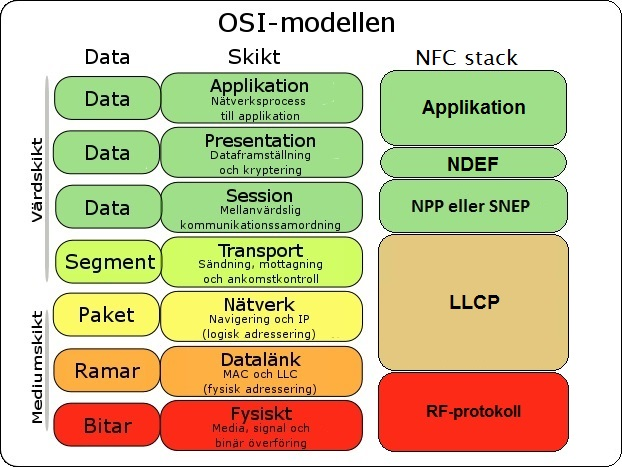
\includegraphics[scale=0.7]{NFC_stack}
% bild in här
\begin{figure}[H]
\centering
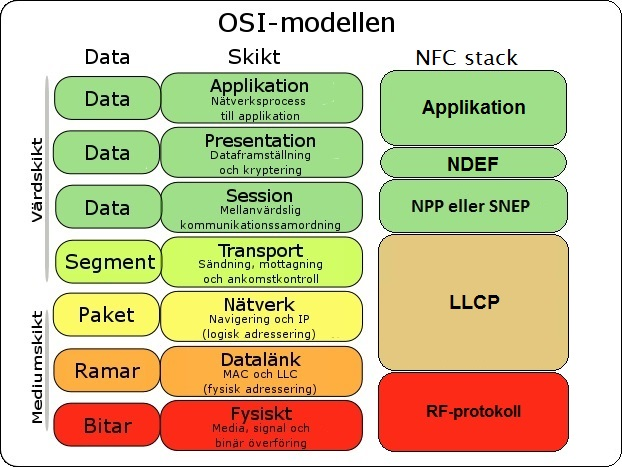
\includegraphics[scale=0.7]{NFC_stack.jpg}
\caption{Här visas NFC-stackens protokoll i förhållande till vilken del i OSI-modellen de utgör.}
\label{fig:NFC Stack}
\end{figure}

\paragraph{NDEF}

\textit{(NFC Data Exchange Format)}[källa] är särskilt utformat för att kunna kapsla in applikationsdata på ett effektivt sätt med minimal overhead. NDEF meddelanden byggs upp av \texttt{records}, vilket kan liknas vid sidor i en bok, där boken utgör NDEF meddelandet. Meddelandet kan bestå av ett obegränsat antal records som alla kan bära på olika sorters data.  

När en applikation önskar sända data över en NFC-länk, kapslas datan in i ett NDEF meddelande, som visas i tabell \ref{tab:NDEF Message}. Beroende på datans storlek och struktur skapas varierande mängd records som tillsammans bildar ett NDEF meddelande. Meddelandet överförs sedan till målenheten som tar emot och behandlar det. NDEF garanterar inte att leverans av data är tillförlitlig och specificerar således inte vad målenheten skall göra vid mottagandet av ett felaktigt utformat NDEF meddelande. Detta lämnas till brukande applikationer att komplettera med datagarantier och felhantering som gemensamt brukar kallas QOS (Quality Of Service).

%Bild
%Bildtext: Ett NDEF meddelande består av en eller flera  records.


\begin{table}
\centering
\begin{tabular}{ |c|c|c|c|c|c|c| }
\hline
\multicolumn{7}{|c|}{\textbf{NDEF Message}} \\
\hline
R\textsubscript{1}MB=1 & ... & R\textsubscript{r} & ... & R\textsubscript{s} & ... & R\textsubscript{t}ME=1 \\
\hline
\end{tabular}
\caption{Ett NDEF meddelande består av en eller flera  records.}
\label{tab:NDEF_Message}
\end{table}


Varje record utformas efter en fördefinerad struktur och består av ett antal fält. Det första fältet är en \texttt{header}, som sedan följs av \texttt{type length, payload length, ID length, type, ID} och till sist \texttt{payload}.

%Bild
%Bildtext: Record layout.

\begin{figure}[H]
\centering
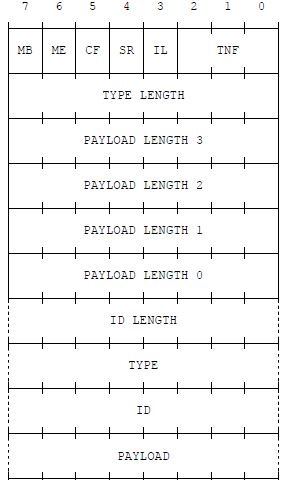
\includegraphics[scale=0.7]{NDEF_record_layout.jpg}
\caption{Record layout.}
\label{fig:record_layout}
\end{figure}

\begin{itemize}
\item \textbf{Header.} En record header är en byte lång där varje bit har olika betydelser.
\begin{itemize}
\item Den första biten är MB som är en förkortning av message begin vilken indikerar att detta är den första record i NDEF meddelandet. Denna bit är ettställd i första record, nollställd i övriga.
\item Den andra biten är ME som är en förkortning av message end vilken indikerar att detta är sista record i NDEF-meddelandet. Denna bit är endast ettställd i sista record, nollställd i övriga.
\item Den tredje biten är CF som är en förkortning av chunk flag vilken och indikerar att NDEF-meddelandet är chunked. Chunk-mekanismen tillåter att ett stort datapaket delas upp över flertalet record. Denna mekanism kommer inte att behandlas i denna text då den utvecklade mjukvaran inte nyttjar detta.
\item Den fjärde biten är SR som är en förkortning av short record vilken används då en mindre mängd data skall överföras. När SR biten är ettställd minskas mängden payload length fält från 4 till 1.
\item Den femte biten är IL vilken indikerar huruvida ID length fältet existerar i record.
\item De sista bitarna, bit 6 till 8, bildar TNF vilken är en förkortning av type name format och definerar strukturen av type-fältet i record.
\end{itemize}
\item \textbf{Type Length.} Definerar hur många bytes som utgör Type-fältet.
\item \textbf{Payload length 0-3.} Varje delfält i payload är en byte stor vilket ger payload length fältet en total storlek på 4 bytes. Payload length indikerar storleken på payload fältet som huserar applikationsdatan. I en record med SR nollstäld kan payload- fältet vara  $8*2^8$ bytes stort, det vill säga 4,29 gigabytes. Med SR ettställd kvarstår enbart ett payload lenght-fält vilket ger  payload-fältet en maximal storlek på 255 bytes.
\item \textbf{Type.} Detta fält definerar vilken typ av data som payload-fältet innehåller. Kraven vad gäller struktur och kodning som specificerats av TNF fältet i header måste följas. Värdet på detta fält kan underlätta behandlingen av applikationsdatan hos målenheten, dock specificeras det inte hur behandlingen sker utan det är upp till applikationen att implementera.
\item \textbf{ID.} Värdet på detta fält är unikt och utgör en unik identiferare kallad URI. Records kan således skiljas åt genom att studera värdet av URI och NDEF garanterar att detta nummer är unikt genom att tillhandahålla en generator.
\item \textbf{Payload.} Detta fält huserar applikationsdata.
\end{itemize}
I figur \ref{fig:NDEF_Message_example} ges ett exempel på ett NDEF-meddelande som kommer att följa med till andra avsnitt som behandlar NFC-stacken.

\begin{figure}[H]
\centering
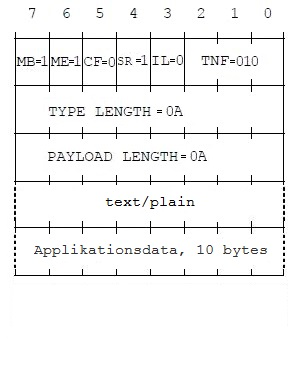
\includegraphics[scale=0.7]{NDEF_Message_example.jpg}
\caption{Exempel på ett NDEF Message.}
\label{fig:NDEF_Message_example}
\end{figure}

(Använd referens istället för "nedan"!!!!!!!!!!!!!!!!!!!!!!!)

%bild

\paragraph{SNEP} 
(Simpel NDEF exchange protocol)[källa] är det protokoll i NFC-stacken som hanterar utbytet av NDEF-meddelanden. SNEP är ett så kallat request/response protokoll, en klient skickar en SNEP-förfrågan till en server som, beroende på förfrågans innehåll, returnerar ett passande svar om det erfodras.

\subparagraph{Förfrågningar}
SNEP har specificerat förfrågningens utseende som visas i figur \ref{fig:SNEP_request_message}:

%bild
\begin{figure}[H]
\centering
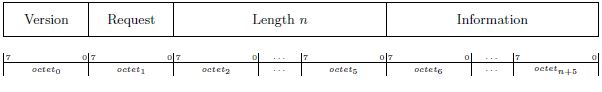
\includegraphics[scale=0.8]{SNEP_request_message.jpg}
\caption{SNEP request message.}
\label{fig:SNEP_request_message}
\end{figure}

\begin{itemize}
\item \textbf{Version.} Detta fält definerar vilken version av SNEP som förfrågan bygger på. Versionsfältet är indelat i två delfält kallat Major och Minor om 4-bit vardera där Major huserar heltalet av versionsnummret och Minor huserar decimaldelen av versionsnummret. För att en kunna genomföra en SNEP session måste klient och server förstå varandra och deras förmåga att förstå varandra avgörs av versionsfältet. Vid mottagande av en SNEP förfrågan kontrollerar servern versionsnumret. Stämmer numret helt överens med den version som servern brukar kan SNEP sessionen fullbordas. Stämmer Major delen men inte Minor är det möjligt att slutföra sessionen om servern anpassar sig efter klienten. Skiljer sig Major delen kan sessionen inte genomföras och servern ger avslag.
\item \textbf{Request.} Request - fältet är 8 bitar stort och anger vilken typ av förfrågan det rör sig om. Fältet innehåller koder som alla är\\ förfrågningsrelaterade. Olika förfrågan erfodrar olika svar från servern.
\item \textbf{Length.} Detta fält anger hur många bytes som utgör informationsfältet. Length-fältet är 4 bytes långt vilket resulterar i att informationsfältet som störst får vara 4.29 gigabytes.
\item \textbf{Information} Innehållet i detta fält beror på innehållet i Request-fältet dvs vilket sorts förfrågan det är. I regel är det ett NDEF meddelande som huseras i information-fältet.
\end{itemize}

De förfrågningar en klient kan begära från en server är Continue, Get, Put samt Reject. De två vanligaste förfrågninarna och de vilka är av relevans för projektet är Put och Get vars betydelse och användning förklaras nedan:

\textbf{Put.} En Put-förfrågan har hexadecimal kod 0x02. Klienten ber servern att ta emot det inkapslade NDEF meddelandet och inget svar erfodras av servern.  Put-förfrågan följer den generella utformningen av ett SNEP förfrågan:

%bild
\begin{figure}[H]
\centering
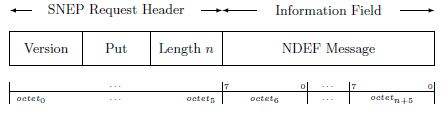
\includegraphics[scale=0.8]{SNEP_put_request.jpg}
\caption{SNEP put request.}
\label{fig:SNEP_put_request}
\end{figure}

\textbf{Get.} En Get-förfrågan har hexadecimal kod 0x01. Klienten ber servern att returnera information inkapslat i ett NDEF meddelande. Vilken information som klienten vill få från servern specificeras i NDEF-meddelandet som huseras i Get-förfrågans information-fält. 

%bild
\begin{figure}[H]
\centering
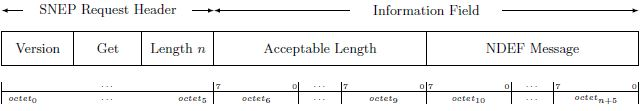
\includegraphics[scale=0.8]{SNEP_get_request.jpg}
\caption{SNEP get request.}
\label{fig:SNEP_get_request}
\end{figure}

Get-förfrågan skiljer sig från den generella förfrågningsstrukturen. Ytterligare ett fält förekommer, Acceptable Length, vars betydelse är att det anger hur stort NDEF-meddelandet i svarsmeddeleandet maximalt får vara. Acceptable length-fältet är 4 bytes vilket gör Get-förfrågan större än en generell förfrågan.

\subparagraph{Svarsmeddelanden}
SNEP har också specificerat svarets utseende:

%bild
\begin{figure}[H]
\centering
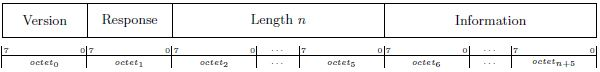
\includegraphics[scale=0.8]{SNEP_response_message.jpg}
\caption{SNEP response message.}
\label{fig:SNEP_response_message}
\end{figure}

Fälten i svaret fyller samma funktion som i förfrågningen men med mindre skillnader.

\textbf{Response.} Fyller samma funktion som Request-fältet. Dock innehåller denna andra koder som alla är av svarstyp.

SNEP svar följer ganska sällan det fördefinerade utseendet. Det är enbart svar på Get-förfrågningar som fullt ut följer det generella utseendet hos ett svar. Vanligt förekommande svar är följande.

\begin{itemize}
\item \textbf{Success.} Detta svar indikerar att servern klarat av att genomföra klientens Get eller Put förfrågan. Utformningen på Success-svaret skiljer sig beroende på om det ges som svar på en Get eller Put förfrågan. I fallet Get följer svaret den generella utformningen med response satt till 0x81 vilket indikerar success. I information-fältet huseras NDEF-meddelandet som ges som svar på Get-förfrågan. I fallet Put sätts response till 0x81, men informations-fältet närvarar ej.
\item \textbf{Not found.} Detta svar ges om servern inte klarar av att returnera önskat svar till klienten. Svarskoden är 0xC0 och inget information-fält förekommer.
\item \textbf{Bad request.} Ges om förfrågningen inte följer fördefinerat utseende. Svarskoden är 0xC2 och inget information-fält förekommer.
\item \textbf{Not implemented.} Detta svar ges om servern inte stödjer den funktionaliet som klienten ber om i förfrågan. Detta svar lämpar sig väl om felaktig request-kod angivits i förfrågan. Inget information-fält förekommer.
\item \textbf{Unsupported version} Ges då klientens SNEP version inte stämmer överens med vad servern kan hantera. Major-delen av version-fältet skiljer sig åt alternativt klarar servern inte av att överbygga de skilnader som olika Minor-värden medför. Inget information-fält förekommer.
\end{itemize}

Alla NFC-enheter har som krav att ha en SNEP-server process körandes. På så vis garanteras att all SNEP kommunikation behandlas. Denna garanti förenklar för både ovanliggande applikationslager som underliggande LLC-lager.

\paragraph{LLCP}
LLCP(Logical Link Control Protocol)[källa] är protokollet som sköter samtliga datalänkar med andra NFC enheter. För att öka överskådligheten hos protokollet har det delats upp i fyra centrala delar: Media access mappning, länkhanteraren, förbindelselös transport och förbindelseorienterad transport. NFC-stacken ser med dessa delar ut som figuren nedan visar.

%bild
\begin{figure}[H]
\centering
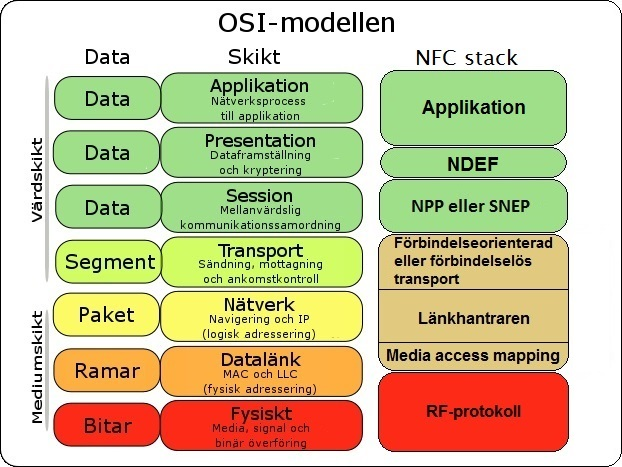
\includegraphics[scale=0.8]{NFC_stack_detail.jpg}
\caption{NFC stack.}
\label{fig:NFC_stack_detail}
\end{figure}

\subparagraph{Media access mappning}
Knyter samman ovanliggande protokoll med de RF-protokoll, vilka styr tekniken som står för den faktiska överföringen av data mellan två NFC enheter. 

\subparagraph{Länkhanteraren}
Detta är en process som styr all NFC-kommunikation och körs på samtliga enheter som stödjer NFC. Länkhanteraren serialiserar all kommunikation till och från NFC-enheter samt kan hantera flera parallella datalänkar och sköta övervakningen av deras aktuella tillstånd.

Ytterligare en viktig funktion som länkhanteraren fyller är att genomföra ett så kallat symmetriförfarande, vilket gör datakanalerna asynkront balanserade. Eftersom NFC är halvt duplex, dvs kommunikation kan ske i båda riktningar men endast en part i kommunikationen får sända samtidigt, måste länkhanteraren hålla reda på vem som har rätten att sända. Under ett normalt utbyte åstadkommes en balans i kommunikationen genom att parterna sänder en LLCP-ram var. Om endera part har rätten att sända, men inte har något att sända, genomför länkhanteraren symmetriförfarandet genom att skicka en speciell LLCP-ram (SYMM) och rätten att sända överlämnas. Symmetriförfarandet gör det möjligt att upptäcka länkförluster som uppkommer av att t.ex kommunikationsavståndet blivit för stort. Om en part i kommunikationen förs utom räckhåll upptäcks detta genom att all form av svar uteblir, dvs varken en normal ram eller en SYMM-ram når målet.

LLCP erbjuder två alternativa transporttjänster till det ovanliggande applikationslagret, förbindelseorienterad transport och förbindelselös transport.

\subparagraph{Förbindelselös transport}
Förbindelselös transport skickar onumrerade datapaket och ger inga garantier till sändande applikation att data tas emot av mottagaren. Mindre kontroll av datatrafiken leder till minskad overhead och därigenom till en snabbare transport. Denna typ av transport lämpar sig således för applikationer som lägger stor vikt på snabbhet och som inte kräver några transportgarantier alternativt implementerar dessa själv. En datalänk av denna sort kallas för logisk datalänk och karaktäriseras av addresserna som den sändande (SSAP) och motta applikationen (DSAP) använder.

\subparagraph{Förbindelseorienterad transport}
Förbindelseorienterad transport skickar numrerade datapaket och garanterar applikationer säker leverans av data men till en kostnad av ökad overhead. Förbindelseorienterad transport lämpar sig för applikationer som ställer högre krav på säkerhet än snabbhet. Två för NFC centrala protokoll, SNEP samt NPP, använder denna transportmetod.

En datalänk av denna typ kallas för uppkoppling. En uppkoppling karaktäriseras av SSAP och DSAP men också ett virtuellt tillstånd som bestäms av fyra stycken numeriska variabler vars olika värden definerar tillståndet. Samtliga variabler kan anta ett värde 0-15 (modulo 16) och syftar till att garantera säker transport av data. Denna mekanism kallas också för ACK från engelskans aknowledgement.

\begin{itemize}
\item \textbf{VS} Första variabeln, sändvariabeln. VS står för hur många numrerade paket, även kallat ramar, som har skickats från enheten över aktuell uppkoppling.
\item \textbf{VSA} Andra variabeln, sändbekräftelsevariabeln. VSA anger senast mottagna numrearad ram som målenheten tagit emot.
\item \textbf{VR} Tredje variabeln, mottagningsvariabeln. VR indikerar vilket nummer som nästa numrearad ram länkhanteraren väntar på att ta emot på aktuell uppkoppling.
\item \textbf{VRA}Fjärde och sista variabeln. VRA står för senast sända VR i en numrerad ram.
\end{itemize}

Utöver dessa variabler håller också länkhanteraren reda på lokalt mottagningsfönster RWL och mottagningsfönstret i målenheten RWR som båda står för hur många numrerade ramar som får skickas mellan enheterna utan att VSA uppdateras. Att VSA inte behöver uppdateras efter varje sändning syftar till att minska behovet av att skicka bekfäftelseramar och overheaden på uppkopplingen minskas.

Ack mekanismen går till på så vis att VS och VR skickas med i varje numrerad ram. VRA sätts till det senast sända VR numret. Vid mottagande av en numrerad ram kontrolleras medföljande VR, VSA sätts till VR -1 då VR implicit indikerar att alla tidigare paket tagits emot korrekt. Vid avikelser, eg om VR i en mottagen ram inte stämmer överens med VSA har ett fel uppstått. Uppkopplingen stängs då ner.

vad händer om fel? FMRMRMFMRM ram skickas med massa satans felkoder. Ta med?

\subparagraph{LLCP-meddelanden}
Eftersom NFC körs på flertalet olika enheter som skiljer sig åt vad avser mjuk- och hårdvara måste LLCP vara flexibelt nog för att kunna köras oberoende av plattform. Denna flexibilitet erhålles genom att specifika parametrar för en datakanal kan förhandlas fram mellan de två kommunicerande LLC-processerna. Viktiga parametrar som är förhandlingsbara är MIU och LTO. 

MIU är en förkortning av Maximum Information Unit och indikerar hur stor ett datapaket maximalt får vara som skall skickas på datalänken. Detta tillåter enheter med begränsade databuffertar att bruka LLCP. Om denna parameter utelämnas i förhandlingen antags ett standardvärde på 128 byte. 

LTO står för Link time Out och indikerar hur länge en länk kan vara inaktiv innan den betraktas som förbrukad och stängs ner. Genom att anpassa LTO kan enheter med låg beräkningskapacitet använda LLCP och kommunicera via NFC, vilket är fallet för ATMEL baserade Arduino-plattformar. Denna parameter utbytes efter att en datalänk etablerats alternativt innan om NFC-enheterna stödjer detta.

LLCP datapaket för förbindelseorienterad transport: 

%bild
\begin{figure}[H]
\centering
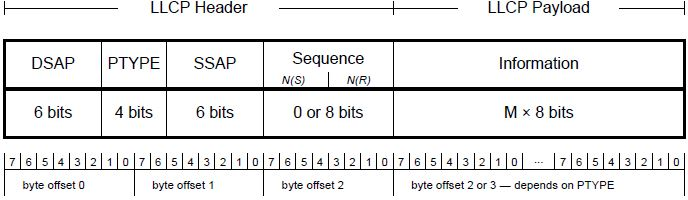
\includegraphics[scale=0.7]{LLCP_datapaket.jpg}
\caption{LLCP datapaket.}
\label{fig:LLCP_datapaket}
\end{figure}

\begin{itemize}
\item \textbf{SAP:} Förkortning av Service Accsess Point och används som addresser vid kommunikation mellan två LLC processer. SAP kan liknas vid en brevlåda i vilken applikationer lämnar meddelanden (data) som den önskar att överföra till en applikation som kör på målenheten. Till varje SAP hör exakt en applikation. 
\item \textbf{DSAP:} Detta fält utgör adressen som addministreras av mottagar LLC vilken sändaren önskar att upprätta en kommunikation-session med. Skall användas som SSAP när ett eventuellt svar ges på det mottagna datapaketet.
\item \textbf{SSAP:} Anger vilken SAP som applikationen blivit tilldelad skickar från. Skall användas som DSAP när ett eventuellt svar ges på det mottagna datapaketet.
\item \textbf{PTYPE:} Detta fält anger vilken sorts datapaket det är och formen på den. Alla datapaket är inte utformade  på exakt samma sätt då de är avsedda för olika ändamål.
\item \textbf{Sequence:} Detta fält är indelat i två stycken underliggande fält. N(S) är här samma nummer som VS. N(S) innehåller således en siffra 0-15 som visar vilket sändnummer ramen har den lokala LLC processen. N(R) är samma som VR. N(R) innehåller alltså en siffra 0-15 som visar vilket nummer som den lokala LLC processen väntar på att ta emot. Sequence-fältet finns enbart med i de ramar som är numrerade. Sekvensnumret används i LLC protokollets ACK mekanism.
\item \textbf{Information:} Innehåller data från ovanliggande lager, t.ex SNEP eller NPP som i sin tur kapslar in applikationsdata. Alternativt kan informationsfälltet innehålla LLC specifika parametrar. Vad informations-fältet innehåller kan utläsas av PTYPE-fältet.
\end{itemize}

Nedan följer ett urval av de typer av datapaket vilka anses vara relevanta för projektet.

\textbf{Connect}

%bild
\begin{figure}[H]
\centering
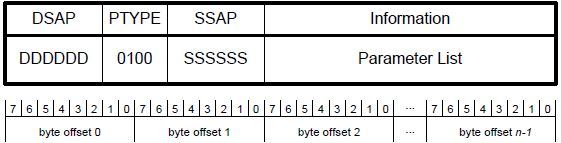
\includegraphics[scale=0.8]{LLCP_connect.jpg}
\caption{LLCP connect.}
\label{fig:LLCP_connect}
\end{figure}

Denna ram används när en NFC-enhet vill etablera en uppkoppling till en annan enhet. DSAP sätts till en välkänd SAP, som t.ex 0x04 vilket indikerar att sändaren vill etablera en uppkoppling med SNEP-servern som kör på målenheten. Alternativ kan SSAP sättas till 0x01 vilken indikerar att målenheten vid mottagande av denna connect-ram skall köra service discovery protocol (SDP) för att hitta en lämplig SAP. SSAP sätts till det värde applikationen som vill utväxla data över NFC blivit tilldelad. Observanta läsare lägger märke till att sequence-fältet inte finns i en Connect-ram. Detta beror på att en Connect-ram är onumrerad, vilket är fallet för många LLCP-ramar. Informationsfältet specificeras till att innehålla datalänkspecifika parametrar. Genom att undersöka PTYPE-fältet kan mottagaren utläsa vilka fält som skall närvara och vad dess innehåll betyder.

\textbf{Connection Complete}

%bild
\begin{figure}[H]
\centering
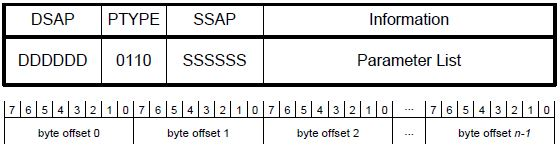
\includegraphics[scale=0.8]{LLCP_connect_complete.jpg}
\caption{LLCP connect complete.}
\label{fig:LLCP_connect_complete}
\end{figure}

Denna ram skall ges som svar på en Connect-ram om en uppkoppling kan upprättas. DSAP sätts till Connect-ramens SSAP värde. SSAP sätts antingen till det värde som SDP returnerat, eller till det fördefinerade värdet som sändaren angav i DSAP. Precis som Connect-ramen är denna ram onumrerad och dess informationsfällt innehåller datalänks-specifika parametrar.

\textbf{DM}

%bild
\begin{figure}[H]
\centering
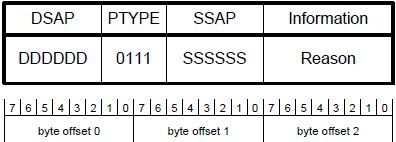
\includegraphics[scale=0.8]{LLCP_DM.jpg}
\caption{LLCP DM}
\label{fig:LLCP_DM}
\end{figure}

Denna ram ges som svar på en Connect-ram när en uppkoppling inte kan etableras. Ramens betydelse är att LLC processen som skickar den inte längre lyssnar på uppkopplingen, den är logiskt avslutad. Anledningen till att uppkopplingen blivit avslutad ges i informations-fälltet. Ramen används också vid avslutande av uppkopplingen och skickas då som svar på en DISC-ram.

\textbf{Information}

%bild
\begin{figure}[H]
\centering
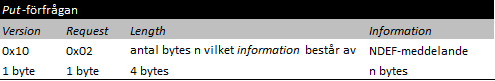
\includegraphics[scale=0.7]{LLCP_information.png}
\caption{LLCP information.}
\label{fig:LLCP_information}
\end{figure}

När utbytet av Connect-ramen och CC-ramen genomförts är uppkopplingen etablerad. Utbytet av applikationsdata kan inledas. Informations-ramen är ramen som är ämnad för att överföra data mellan två NFC-enheter. För att kunna upptäcka eventuell dataförlust är denna ram numrerad. Informationsfältet innehåller i detta fall data från ovanliggande applikationer.

\textbf{Symmetry}

%bild
\begin{figure}[H]
\centering
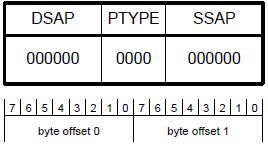
\includegraphics[scale=0.8]{LLCP_symmetri.jpg}
\caption{LLCP symmetri.}
\label{fig:LLCP_symmetri}
\end{figure}

Denna ram används i den tidigare beskrivna symmetri-proceduren för att undvika länk-timeout under pågående kommunikation. När en NFC-enhet har exklusiv rätt att skicka data men saknar något att skicka och önskar bibehålla datalänken genomförs symmetri-proceduren under vilken denna ram spelar en central roll.

%bild
%bildtext
\begin{figure}[H]
\centering
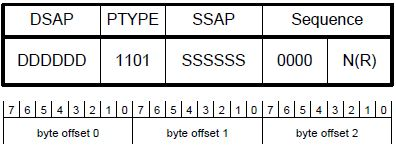
\includegraphics[scale=0.8]{LLCP_ack.jpg}
\caption{LLCP ACK-ram}
\label{fig:LLCP_ack}
\end{figure}

Denna ram används för att indikera att föregående frame togs emot korrekt när ingen nyttig data kan skickas. Detta är således LLC protokollets dedikerade ACK-ram.

\textbf{DISC}

%bild
\begin{figure}[H]
\centering
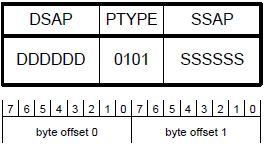
\includegraphics[scale=0.8]{LLCP_DISC.jpg}
\caption{LLCP DISC}
\label{fig:LLCP_DISC}
\end{figure}

Används när en av parterna vill stänga ner datalänken. När en LLC process tar emot en ram av denna typ kommer den inte att skicka mer data över denna uppkoppling. Kanalen stängs ned först när sändande part mottager ett svar i form av en DM-ram.


\paragraph{RF-protokoll}
De RF-protokoll vilka det utvalda NFC-chippet PN532 från NXP Semiconductors implementerar är ISO/IEC 18092 NFCIP-1(Near Field Communication – Interface And Protocol)[7] samt ISO/IEC 14443 där det förstnämnda används i samband med kommunikation mot en aktiv NFC-enhet. NFCIP-1 är således det protokoll detta projekt nyttjar hos NFC-chippet och detta specifiserar bland annat moduleringstekniker, kodningsanvisningar, överföringshastigheter, datakollisionskontroll och ram-format. Vidare definierar NFCIP-1 initieringsförfarandet, datautbytesförfarandet (DEP) och deaktiveringsförfarandet vilket används vid aktiv kommunikation.

\subparagraph{Initieringsförfarandet}
I initieringsförfarandet sänds en \texttt{ATR\_REQ} från den initierande enheten till målenheten, vilken sänder tillbaka en ATR\_RES som svar. En ATR\_REQ och en ATR\_RES är snarlikt uppbyggda och beskrivs samtidigt i följande stycke.

De två första bytesen utav en \texttt{ATR\_REQ} eller \texttt{ATR\_RES}(se figur R) är $0xD4$ och $0x00$, sedan följer NFCID3 vilket är ett slumpartat identifikationsnummer vilket ska vara detsamma under en och samma kommunikations-session. Följande fem bytes i en ATR\_RES respektive fyra bytes i en ATR\_REQ (TO uteblir), är parametrar vilka sköts av NFCIP-1. Slutligen följer så kallade generella bytes vilka inleds med de magiska LLCP nummren och efter dem radas de TLV parametrar(se 3.1.1.3) upp som önskar utbytas i initieringsförfarandet.

%bild
\begin{figure}[H]
\centering
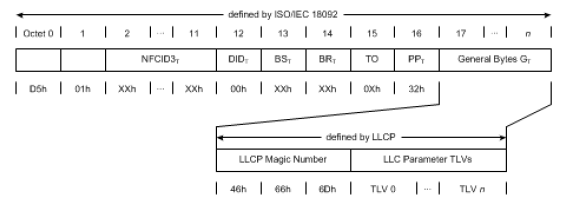
\includegraphics[scale=0.8]{LLCP_ATR_RES.png}
\caption{Utförandet av en ATR\_RES. Bildkälla LLCP}
\label{fig:LLCP_ATR_RES}
\end{figure}

\subparagraph{Datautbytesförfarande}
DEP(Data Exchange Protocol) är det protokoll som följs vid utbytandet av data mellan två aktiva NFC enheter på RF-protokolls-nivå och är ett blockorienterat transportprotokoll med inbyggd felhantering och kedjemekanism. Denna mekanism används då den data vilken ska överföras inte får plats i en ram.

\subparagraph{Deaktiveringsförfarande}
RELEASE/deaktivering

\paragraph{Ett typiskt kommunikationsförlopp}
\subparagraph{Uppkopplingsupprättande}
En applikation som körs på en NFC-enhet önskar att skicka data till en annan applikation som körs på en målenhet. För att kunna sända datan måste LLC processen på den sändande enheten först upprätta en uppkoppling genom att skicka en Connect-ram. PTYPE sätts till 0100 vilket indikerar en Connect-ram. Connect-ramens SSAP sätts till den address som aktuell applikation blivit tilldelad. På samtliga NFC-enheter körs en SNEP-server. Denna server använder en välkänd SAP (0x04) och det är denna SAP som används som DSAP i Connect-ramen om applikationsdatan skall utväxlas med SNEP vilket ofta är fallet. 

När LLC processen på målenheten mottager en Connect-ram, och DSAP och SSAP är giltliga, bearbetas de uppkopplingsspecifika parametrana som eventuellt medföljde Connect-ramen. Avsedd applikation, i detta fall SNEP-servern, meddelas om att någon önskar utbyta data. SNEP-servern kontrollerar huruvida datautbyte är möjligt. Är datautbyte inte möjligt meddelas LLC processen som då sänder en DM-ram och uppkopplingen avslutas. Är utbyte av data möjligt meddelas LLC om detta som då skickar en CC-ram. I denna ram sätts DSAP till Connect-ramens SSAP och SSAP till Connect-ramens DSAP. VS, VR, VSA och VRA är samtliga satta till 0.

Vid mottagandet CC-ramen sätter den sändande LLC processen VS, VR, VSA och VRA är samtliga satta till 0. Uppkopplingen är etablerad och kommunikationen övergår i informationsutbytesfasen.

\subparagraph{Informationsutbyte}
Den lokala LLC processen sänder  iväg den första Informations-ramen som kapslar in applikationsdata. Eftersom det är den första informations-ramen sätts sekvensnummret N(S) och N(R) till 0. Om ytterligare informations-ramar skickas ökas successivt sekvensnummret VS och N(S). Informationsfältet innehåller SNEP-ramen som i sin tur innehåller datan som skall överföras.

Vid mottagande av informations-ramen erhålls den inpackade SNEP-ramen som levereras till SNEP-servern. Om applikationen på målenheten önskar svara kapslar LLC processen på målenheten in svaret i en information-ram med sekvensnummret N(S) = 0 och N(R) = 1. Det första indikerar att detta är den första informations-ramen som målenheten skickar till sändarenheten, det senare indikerar att föregående informations-ram tagits emot korrekt. Om inget svar ges skickar LLC-processen på målenheten en RR-ram med sekvensnummer N(R) = 1 som fyller samma funktion som informationsramen-ramen men utan medföljande data. Datautbytet fortlöper med successivt ökande tillståndsvariabler tills antingen ett fel uppstår eller tills utbytet är färdigt. Båda resulterar i att kommunikationen övergår i uppkopplingsavslutningesfasen.

\subparagraph{Uppkopplingsavslutning}
Applikationen signalerar den lokala LLC processen om att utbytet är färdigt. Den lokala LLC processen skickar då en DISC-ram till LLC-processen på målenheten. LLC processen på den sändande enheten slutar ta emot samtliga ramar förutom en DM-ram. Vid mottagande av denna DM-ram avslutas uppkopplingen. 
Vid mottagande av DISC-ramen ses uppkopplingen som avslutad av LLC processen på målenheten. Processen meddelar SNEP-servern om att uppkopplingen stängs ned och skickar en sista DM-ram över uppkopplingen.

Båda parterna ser nu uppkopplingen som avslutad.


\subsubsection{Säkerhet}
Detta avsnitt är baserat på artikeln Strengths and Weaknesses of Near Field Communication (NFC) Technology[14].

NFC har likt RFID i sitt grundutförande inga inbyggda säkerhetsfunktioner som förhindrar avlyssning, modifiering eller utstörning av kommunikationen. Eftersom kommunikationen är trådlös så kommer avlyssning alltid att vara möjligt och det är upp till sändare och mottagare att kryptera meddelanden om behovet finns. Följande sektioner beskriver hur dessa säkerhetsbrister kan åtgärdas. 

\paragraph{Tjuvlyssning}
Eftersom NFC är trådlös kommunikation som skickar information via radiovågor kan icke avsedda enheter fånga upp signalerna. För att kunna fånga upp signalerna måste dessa icke-avsedda enheter befinna sig inom kommunikationsräckhåll. På grund av NFCs korta kommunikationsavstånd, kring 10 centimeter, besitter NFC ett inneboende skydd mot avlyssning. Avlysstningsutrustningen måste föras väldigt nära de kommunicerande enheterna vilket underlättar upptäckten av avlyssning. Det finns dock ingen garanti för att signalerna kan fångas upp på betydlig längre avstånd eftersom flertalet parametrar spelar in i hur lång radiovågor kan färdas. Viktigast av dessa är:

\begin{itemize}
\item Antenn
\item Effekt
\item Moduleringsteknik
\item Omgivning
\end{itemize}

Vilken antenn som sändare och avlyssnare använder spelar en avgörande roll. Dess dimensioner, utformning och omslutande material är några viktiga faktorer som spelar i hur väl en antenn kan sända och ta emot radiovågor. I t.ex telefoner används en relativt liten spole vilket starkt begränsar signalstyrkan. Vidare så är telefoner i dagsläget ofta innesluten i robust plast eller aluminium som också minskar signalsstyrkan.

Effekten som signalen sänds med avgör hur långt de kan färdas. En signals effekt är starkt sammankopplad med bärvågens amplitud. Ju större amplitud bärvågenvågen har dessto större effekt har signalen. En signal som sänds med hög effekt och följaktligen stor amplitud kan färdas längre än en signal som sänds med låg effekt och som har liten amplitud. 

Moduleringstekniken, enkelt uttryckt hur informationen mönstras in i bärvågen, är också avgörande i sammanhanget. Olika moduleringstekniker medför olika mönster i bärvågen. Hur kraftig modulering som används uttrycks i procent och symboliserar hur tydligt mönster informationen resulterar i. NFC bygger på amplitudmodulering vilket innebär att informationen mönstras in som amplitudvariationer. I detta sammanhang betyder alltså kraftig modulering hur stora amplitudvariationer hos bärvågen som informationen kodas med. Kraftig modulering uppåt 100\% innebär att bärvågen stundom helt släcks ut. Svagare modulering kring 10\% innebär mindre variationer i amplitud hos bärvågen. Det följer att olika moduleringstekniker med olika kraftfull modulering resulterar i signaler med olika egenskaper varav en, hur långt signalen effektivt kan bära information, är relevant i detta sammanhang.

Omgivning spelar en avgörande roll i hur långt radiosignaler kan färdas. Inne i en byggnad finns väggar och andra föremål vilket kraftigt begränsar signalens förmåga att breda ut sig. Bakgrundsbrus, andra radiovågor från telefoner, radioapparater och övrig elektronik, stör ut signalen och minskar signalens räckvidd.

Alla dessa faktorer gör att det inte är känt vilka avstånd avlyssning kan genomföras på, men experiment har genomförts med framgång på avstånd uppåt 10 meter. 


\paragraph{Datamodifiering}
Datamodifiering går ut på att en attackerande enhet försöker störa kommunikationen mellan två NFC-enheter genom att modifiera informationen som skickas mellan enheterna. I sin enklaste form går datamodifiering ut på att störa ut  informationsbärande signaler. Mer avancerad datamodifiering går ut på att modifiera signalerna och därigenom informationen som sänds mellan enheterna på ett sådant sätt informationen fortfarande uppfattas som korrekt av mottagaren. 

\paragraph{"Man in the middle" attack}
En så kallad man in the middle attack går ut på att en illasinnad enhet agerar mellanhand mellan sändare och mottagare. Sändare och mottagare handlar i god tro om att de talar direkt till varandra. Mellanhanden får tillgång till känslig information och har dessutom möjligheten att ändra innehållet av datan. En attack av detta slag är i praktiken omöjligt att genomföra på en NFC länk oavsett om kommunikationen sker mellan två aktiva enheter eller en aktiv och en passiv enhet. För att kunna posera som sändare måste mellanhanden stundom aktivt störa ut data som parterna försöker utbyta med varandra och andra gånger försöka skapa en signal som perfekt överlappar befintlig signal. Minsta avvikelse i utstörningen eller överlappningen resulterar i att datan som skickas över länken blir förvrängd och om de två enheterna aktivt lyssnar på länken kan denna förvräning relativt lätt upptäckas. 

\subsection{Android}
Enligt Google(2013) är Android världens mest använda operativsystem för mobila enheter. Android är baserat på Linuxkärnan och kan med hjälp av denna stödja många olika typer av hårdvara. Detta gör Android kompatibel med enheter från många olika tillverkare och det är en av anledningarna till att Android har blivit så dominerande. En annan anledning till dominansen är Androids öppna källkod och dess användande av världens mest använda programspråk, Java(Google, 2013).

För att komma igång och skriva applikationer för Android är det några saker en utvecklare behöver känna till. Förutom grundläggande kunskaper inom Java-programmering och mjukvaruutveckling i allmänhet bör en utvecklare av Android-applikationer inneha kunskaper inom i huvudsak tre områden.

Först bör en utvecklare inneha kunskaper om den särskilda livscykel, se bilden nedan, en Android aktivitet har. Livscykeln beskriver de olika tillstånd en aktivitet(fotnot 1) kan befinna sig i samt de olika automatiska anrop som sker då aktiviteten tar sig mellan dem. Livscykeln ger ytterligare funktionalitet men också vissa svårigheter så som att viktiga data måste sparas och återställas när användaren till exempel vrider telefonen.

%bild
%bildtext: Bilden som är publicerad av Google(2013) beskriver en Android aktivitets livscykel. Särskilt beskriver den de olika statusar den kan befinna sig i samt de metodanrop som sker när den tar sig mellan dem.
\begin{figure}[H]
\centering
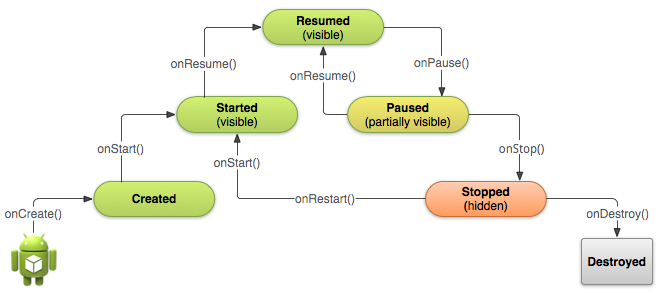
\includegraphics[scale=0.7]{Android_aktivitet.png}
\caption{Bilden som är publicerad av Google(2013) beskriver en Android aktivitets livscykel. Särskilt beskriver den de olika statusar den kan befinna sig i samt de metodanrop som sker när den tar sig mellan dem.}
\label{Fig:Android_aktivitet}
\end{figure}

För det andra måste en utecklare av Android-applikationer ha kunskap om de Android-specifika API som Google tillhandhåller. Dessa API beskriver de funktioner som är unika för Android-enheter. Där beskrivs t.ex. hur ett användargränssnitt byggs upp, hur en lokal databas sätts upp och hur applikationen kommunicerar med andra applikationer och med omvärden. Särskilt användbart för projektet är det API som specificerar kommunikation över NFC.

Vidare bör en utecklare också känna till filstrukturen hos ett Android-projekt, de specifika verktyg för Android-utveckling som finns samt vilka filer som definierar vad. Exempelvis bör kunskap finnas om vilket xml-dokument som definierar vilken vy och hur inställningar påverkar för såväl en aktivitet som för hela applikationen.

\subsubsection{NFC för Android}
Google (2013) skriver att Android innehåller funktionalitet för att kommunicera via NFC mot två huvudsakliga enheter. Dels finns det funktionalitet för att skriva och läsa från taggar och dels finns det funktionalitet för att kommunicera mot andra enheter vilka har Android som operativsystem. Eftersom detta arbete nyttjar kommunikation mellan två aktiva NFC-enheter är det den senare som är mest relevant. Detta eftersom det är en Androidenhet mikrokontrollern imiterar.

Vidare skriver Google(2013) att det är möjligt att skicka vilken typ av meddelande som helst via NFC men att de rekommenderar meddelanden av typen NDEF (NFC Data Exchange Format) vilken är den av NFC Forum definierade standarden. När ett NDEF-meddelande tas emot hanteras det av en process som är ansvarig för att den inkommande datan skickas vidare till rätt applikation. En applikation kan deklarera vilka typer av data den kan ta emot i dess manifest.

För den eftersökta kommunikationen mellan två Androidenheter används en teknik vilken kallas Android Beam(Google 2013). Denna teknik bygger på utbyten av NDEF-meddelanden. Android Beam fungerar genom att två enheter förs mot varandra vilket förbereder skickandet av ett meddelande. Sändningen slutförs genom att användaren trycker på skärmen. Tekniken sker alltså utan att någon form av parning(fotnot 1) behövs så som är fallet i andra kommunikationsmetoder, exempelvis Bluetooth (\url{http://www.cs.utexas.edu/~shmat/shmat_fcs07.pdf}).

Google (2013) gör dess Android Beam teknik tillgänglig via ett antal API. Dessa definierar allt ifrån ihopsättande av ett meddelande till hur systemet automatisk förbereder sändande och mottagande. Första steget i användandet av kommunikation via NFC är att få tag på ett objekt som representerar NFC-hårdvaran. Den representeras som ett objekt av typen NFCAdapter. Objektrepresentationen fås via den statiska metoden getDefaultAdapter.

Vidare kan en aktivitet ställas in för sändning genom att en klass implementerar ett särskilt interface, CreateNdefMessageCallback. Implementationen ger klassen förmågan att dynamiskt skapa och skicka meddelanden via Android Beam. För att sedan möjliggöra sändningen från en aktivitet behöver denna välja den implementerade klassen genom att kalla på metoden setNdefPushMessageCallback. För att ta emot meddelandet behövs, förutom att det står angivit i manifestet, metoden onNewIntent skrivas över och i denna behöver meddelandet fångas upp för att sedan tolkas.

fotnot 1 parning eng Pairing

\subsection{Arduino}
En Arduino är en mikrokontroller, det vill säga en mikroprocessor med tillhörande nödvändig elektronik kopplad till ett flertal in- och utgångar, vilken främst är avsedd för hobbymarknaden. Arduino-plattformen har framställts med användarvänlighet i fokus(Arduino, 2013) och har en stor community online. All den kod vilken bygger upp hela arduino-plattformen är licenserad under antingen GNU General Public License eller GNU Lesser General Public License(Arduinos källkod, 2013) vilket bland annat ger möljlighet för ett arbete av detta slaget att nyttja all denna kod. 

Flertalet modeller i olika storlekar och prestandaklasser finns men en av de vanligare och den modellen vilken kommer beskrivas mer ingånde är Arduino Mega 2560 R3. Denna mikrokontroller baseras på mikroprocessorn ATmega2560 från Atmel(Arduino, 2013) med klockhastigheten 16 MHz. Vidare kan läsas på Arduinos(2013) produktsida att denna enhet innehar 16 analoga ingångar, 54 digitala in/utgångar, 4 UART(Universal Asynchronous Receiver/Transmitter), USB-kontakt, ström-jack, återställningsknapp och en ICSP(In-Circuit Serial Programming) header. Minnesstorleken på flash-minnet är 256 KB, SRAM(Static Random-Access Memory) är 8 KB stort och 4 KB EEPROM(Electrically Erasable Programmable Read-Only Memory) finns.

En mikrokontroller av arduino-typ kan köras med en bootloader(Arduino, 2013) vilket är ett litet förinstallerat program och på Arduino Mega 2560 R3 utgör den omkring 8 KB av flash-minnet. En bootloader är grovt beskrivet ett väldigt litet operativsystem vilken gör exekveringen möjlig av den kod som användaren av mikrokontrollern har laddat in i minnet. 

Arduino-plattformens utvecklingsmiljö är enkel i sitt utförande och programspråket som används är C/C++.  Utvecklingsmiljön innehåller allt som behövs för att en användare ska kunna skriva sin kod för att sedan kompilera och för att slutligen ladda upp koden mot vald Arduino-modell. Tyvärr erbjuder inte utvecklingsmiljön många funktioner där de mest avändbara är auto-formatering och möjligheten att inkludera externa arduino-specifika bibliotek. 

Avsaknad av debug! Och eftersom den är så satans enkel har du ingen vidare insyn i hur koden kompileras och vad som faktiskt läggs på kontrollern.

\subsubsection{Arduino-specifika källkodsbibliotek}
Ett flertal källkodsbibliotek finns till användarens hjälp och nästan alla dessa bibliotek är fokuserade på kommunikation mot kringenheter. Andra bibliotek finns men är då skrivna av användare. De bibliotek som tas upp i detta avsnitt är de bibliotek vilka har använts för implementationen av låsenheten.

För att kommunicera mot kringenheter via kommunikationsprotokollet I2C[källa] behövs källkodsbiblioteket WIRE. Om Arduino-modellen Arduino Mega 2560 R3 används kommer biblioteket använda pinne nummer 20 och 21 för SDA(Serial Data Line) respektive SCL(Serial Clock Line). Dessa pinnar är kopplade till motsvarande pinnar på kringenheten. Att förstå och använda biblioteket är relativt trivialt och tas ej upp i denna text.

%skriv om källkodsbiblioteket AVR/SLEEP

\subsubsection{NFC för Arduino mha PN532 NFC/RFID Shield}
För att en Arduino ska kunna nyttja kommunikation via NFC krävs att en så kallad sköld vilken har NFC-funktionallitet är ansluten till enheten. En sköld av det beskrivna slaget är Adafruits PN532 NFC/RFID Shield som baseras på NFC-chippet PN532 från företaget NXP Semiconductors. 

Skölden kommunicerar mot en mikrokontroller med teknikerna SPI[källa], HSU[källa] eller I2C[källa]. För teknikerna SPI och I2C finns bibliotek att tillgå, skrivna av Adafruit, vilka kontrollerar kommunikationen mellan skölden och mikrokontrollern. Vidare ger också biblioteken ytterligare funktionallitet då manipulation av taggar erbjuds. Dock innehåller biblioteken inte stöd för kommunikation mot en aktiv NFC-enhet(se 3.1 NFC) vilket är det detta arbete önskar nyttja.

De protokoll som PN532 NFC/RFID Shield har implementerade är de RF-protokoll vilka är de som finns längst ner i NFC-stacken(NXP, 2007). Dessa protokoll möjliggör den faktiska överföringen av data och det implementerade protokollet med högst abstraktionsnivå är DEP(Data Exchange Protocol) vilket skriv lite om DEP

För att kontrollera PN532 NFC/RFID Shield finns ett stort antal kommandon vilka beskrivs utförligt i användarmanualen till PN532(NXP, 2007) och de beskrivningar vilka görs i detta avsnitt härör från detta dokument. Ett kommando skickas över vald kommunikationsteknik inkappslad i en ram vilken är specifierad enligt figur X(NXP, 2007). Denna ram inkappslar också de svar som fås från PN532 NFC/RFID Shield. Om inget annat anges består en ruta i detta avsnitts figurer utav en byte.

%bild
%bildtext: figur X. Kommando- och svars-ram Bildkälla PN532 NFC/RFID Shield User manual, översatt till svenska.
\begin{figure}[H]
\centering
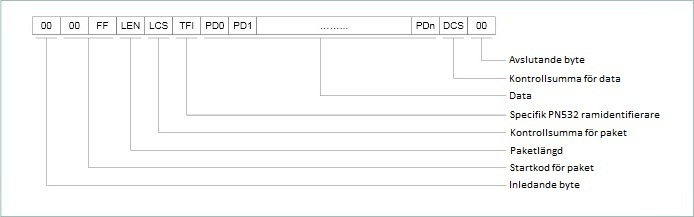
\includegraphics[scale=0.8]{PN532_shield_ram.jpg}
\caption{Kommando- och svars-ram. Bildkälla PN532 NFC/RFID Shield User manual, översatt till svenska.}
\label{fig:PN532_shield_ram}
\end{figure}

\begin{itemize}
\item Inledande bytes. Den byte som inleder en kommando-ram innehåller $0x00$.
\item Startkod för paket. Den består av två bytes innehållande \texttt{0x00} respektive $0xFF$.
\item Paketlängd. En byte vilken indikerar hur många bytes datafältet innehåller, det vill säga från TFI till och med PDn.
Kontrollsumma för paket. En byte innehållande en kontrollsumma vilken satisfierar vilkoret LEN +LCS = $0x00$.
\item Specifik PN532 ramidentifierare. En byte vilken indikerar om PN532 NFC/RFID Shield är sändare eller mottagare.
\begin{itemize}
\item \texttt{0xD4} anger att PN532 NFC/RFID Shield är mottagare av ramen.
\item $0xD5$ anger att PN532 NFC/RFID Shield är sändare av ramen.
\end{itemize}
\item Data. Paketlängd-1 bytes av paketdata vilka sträcker sig från PD0 till PDn. Maximalt kan 262 bytes skickas i en ram till skölden.
\item Kontrollsumma för data. En byte innehållande en kontrollsumma vilken satisfierar vilkoret TFI + PD0 + PD1 + ... + PDn + DCS = 0x00.
\item Avslutande bytes. Den byte som avslutar en kommando-ram innehåller 0x00.
\end{itemize}

(fotnot 1) De bytes som är efter den avslutande byten eller innan den inledande byten kan vara godtyckligt många och ha godtyckliga värden så länge följden 0x00 0xFF inte förkommer.

De kommandon som kan nyttjas grupperas i fyra grupper, generella kommandon, RF-kommunikation, initiator och target. I gruppen generella kommandonfinns kommandon som diagnoserar NFC-chipet, läser och skriver till register samt konfigurerar skölden i viss mån. Gruppen RF-kommunikation huserar två kommandon vilka konfigurerar radio-fältet respektive används för radio-fälts reglering. Tredje gruppen, inintiator, innehåller de kommandon vilka används då PN532 NFC/RFID Shield agerar initiator till NFC-kommunikationen, och den sista gruppen omfattar de kommandon vilka används då PN532 NFC/RFID Shield är målenhet för NFC-kommunikation.

Då PN532 NFC/RFID Shield har mottagit en kommando-ram korrekt sänds en ACK-ram tillbaka till sändaren vilken är uppbyggd enligt figur \ref{fig:PN532_shield_ack}.

%bild
%bildtext: figur Y. Bildkälla PN532 NFC/RFID Shield User manual, översatt till svenska.
\begin{figure}[H]
\centering
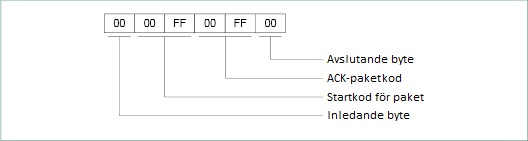
\includegraphics[scale=0.8]{PN532_shield_ack.jpg}
\caption{Ack-ram. Bildkälla PN532 NFC/RFID Shield User manual, översatt till svenska.}
\label{fig:PN532_shield_ack}
\end{figure}


Om en kommando-ram inte mottages korrekt av PN532 NFC/RFID Shield eller om ett fel på applikationsnivå inträffar skickas en ERROR-ram till mikrokontrollern vilken är uppbyggt enligt figur \ref{fig:PN532_shield_error}. är detta rätt!?

%bild
%bildtext: figur Z. Bildkälla PN532 NFC/RFID Shield User manual, översatt till svenska.
\begin{figure}[H]
\centering
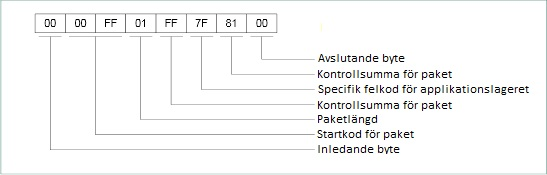
\includegraphics[scale=0.8]{PN532_shield_error.jpg}
\caption{Error-ram. Bildkälla PN532 NFC/RFID Shield User manual, översatt till svenska.}
\label{fig:PN532_shield_error}
\end{figure}


De kommandon som beskrivs i denna text är de vilka varit till nytta för utvecklingen av prototypen och de återstående kommandona tas ej upp, bland annat utelämnas kommandogrupperna RF-kommandon och initiator-kommandon helt då de ej nyttjas. De figurer vilka beskriver 

\paragraph{Generella Kommandon till PN532 NFC/RFID Shield}
Dessa kommandon utför läsningar och skrivningar till register, diagnosering utav NFC-chipet, viss konfiguration av skölden samt att skölden kan ställas i olika vilolägen. 

\subparagraph{SAMConfiguration}
När PN532 NFC/RFID Shield startas upp befinner sig NFC-chippet i läget LowVbat, genom att anropa kommandot SAM(Security Access Module)Configuration(fotnot 1) vaknar skölden och går in i ett läge där den behandlar också alla andra kommandon. Kommandot SAMConfiguration är uppbyggt enligt tabell \ref{tab:SAMConfiguration}, vilken visar fälten TFI, PD0 ända till PDn i en kommando-ram. 

%bild alt. tabell
\begin{table}
\centering
\begin{tabular}{ |c|c|c|c|c| }
\hline
$0xD4$ & $0x14$ & \texttt{Läge} & \texttt{Timeout} & \texttt{[IRQ]}\\
\hline
\end{tabular}
\caption{SAMConfiguration.}
\label{tab:SAMConfiguration}
\end{table}

\begin{itemize}
\item 0xD4 anger att PN532 NFC/RFID Shield är mottagare av ramen.
\item 0x14 är den kommandospecifika koden.
\item Läge. Här väljs hur SAM(Security Access Module) ska användas. Då PN532 NFC/RFID Shield inte har någon SAM väljs normalt läge då en SAM inte används, genom att ange 0x01.
\item Timeout. Om SAM inte används sätts denna parameter till 0x00.
\item IRQ, frivilligt fält. Om en IRQ-lina ska användas för smidigare kommunikationen mot en Arduino anges 0x01, annars 0x00.
\end{itemize}

Svarsmeddelandet till SAMConfiguration är uppbyggt enligt tabell \ref{tab:svar_SAMConfiguration} vilken visar fälten TFI, PD0 ända till PDn i en svars-ram. Det ända som svaret innehåller, förutom TFI,  är den kommandospecifika svarskoden 0x15.

%bild
\begin{table}
\centering
\begin{tabular}{ |c|c| }
\hline
$0xD5$ & $0x15$ \\
\hline
\end{tabular}
\caption{Svarsmeddelande till SAMConfiguration.}
\label{tab:svar_SAMConfiguration}
\end{table}

fotnot 1: Om SAMConfiguration används för att skölden ska gå ur LowVbat läget måste Mode sättas till 0x01.  

\paragraph{Kommandon till PN532 NFC/RFID Shield då enheten agerar målenhet}

Då PN532 NFC/RFID Shield är målenheten för kommunikationen finns ett antal kommandon som är dedikerade för detta ändmål. Dessa kommandon ger bland annat funktionalitet i form av att konfigurera skölden som en målenhet och att sända samt ta emot data.

\subparagraph{TgInitAsTarget}
För att konfigurera PN532 NFC/RFID Shield som en målenhet anropas kommandot TgInitAsTarget enligt tabell \ref{tab:kommando_TgInitAsTarget}, vilken visar fälten TFI, PD0 ända till PDn i en kommando-ram. 

%tabell
\begin{table}
\centering
\begin{tabular}{ |c|c|c|c|c|c|c|c|c|c| }
\hline
$0xD4$ & $0x8C$ & \texttt{Läge} & \texttt{Mifare parametrar} & \texttt{FeliCa parametrar} & \texttt{NFCID3t} & \texttt{LEN Gt} & \texttt{Gt} & \texttt{LEN Tk} & \texttt{Tk} \\
\hline
\end{tabular}
\caption{Anrop med kommandot TgInitAsTarget.}
\label{tab:kommando_TgInitAsTarget}
\end{table}

\begin{itemize}
\item 0xD4 anger att PN532 NFC/RFID Shield är mottagare av ramen.
\item 0x8C är den kommandospecifika koden.
\item Läge. Val av operationsläge. 
\begin{itemize}
\item bit 0 satt indikerar att skölden endast kommer påbörja kommunikation mot passiva NFC-enheter.
\item bit 1 satt indikerar att skölden följer protokollet DEP() och kommer endast påbörja kommunikation om en ATR\_REQ ram mottas.
\item bit 2 satt indikerar att skölden emulerar en tagg av typen ISO/IEC14443-4 och endast kommer påbörja kommunikation om en RATS ram mottas.
\end{itemize}
\item Mifare parametrar, 6 bytes. Parametrar vilka behöver definieras då kommunikation mot en passiv NFC-enhet i 106 Kb/s önskas.
\item FeliCa parametrar, 18 bytes. Parametrar vilka behöver definieras då kommunikation mot en passiv NFC-enhet i 212/424 Kb/s önskas.
\item NFCID3t, 10 bytes, används som svar, ATR\_RES, om ett ATR\_REQ mottas.
\item LEN Gt anger hur många bytes, max 47, Gt består av. 
\item Gt, LEN Gt bytes, anger de generella bytes som används i ATR\_RES.
\item LEN Tk anger hur många bytes, max 48, Tk består av.
\item Tk, LEN Tk bytes, anger de historiska bytes vilka används i ATS när skölden emulerar en tagg av typen ISO/IEC14443-4.
\end{itemize}

Svarsmeddelandet till TgInitAsTarget är uppbyggt enligt tabell \ref{tab:svar_kommando_TgInitAsTarget}, vilken visar fälten TFI, PD0 ända till PDn i en svars-ram. Svaret innehåller TFI, den kommandospecifika svarskoden $0x8D$, en byte vilken indikerar i vilket läge skölden blivit konfigurerad samt det första meddelandet från initiatorn.

%tabell
\begin{table}
\centering
\begin{tabular}{ |c|c|c|c| }
\hline
$0xD5$ & $0x8D$ & \texttt{Läge} & \texttt{Initiatorns meddelande} \\
\hline
\end{tabular}
\caption{Svar till kommandot TgInitAsTarget.}
\label{tab:svar_kommando_TgInitAsTarget}
\end{table}

\subparagraph{TgSetData}
Detta kommando används då data önskas skickas enligt DEP och är uppbyggt enligt tabell \ref{tab:TgSetData}, vilken visar fälten TFI, PD0 ända till PDn i en kommando-ram. Förutom den kommandospecifika koden innehåller ramen de bytes vilka önskas skickas. Observera att maximalt 262 bytes kan skickas åt gången och om fler ska skickas måste också kommandot TgSetMetaData användas.

%tabell
%bildtext: Figur E.
\begin{table}
\centering
\begin{tabular}{ |c|c|c| }
\hline
$0xD4$ & $0x8E$ & \texttt{Utgående data} \\
\hline
\end{tabular}
\caption{TgSetData.}
\label{tab:TgSetData}
\end{table}

Det svar som anhålles från skölden är uppbyggt enligt tabell \ref{tab:svar_TgSetData}, vilken visar fälten TFI, PD0 ända till PDn i en svars-ram. Förutom att svaret innehåller den kommandospecifika svarskoden 0x8F samt TFI finns också ett statusfält vilket indikerar om sändningen utfördes korrekt, vilket indikeras med $0x00$, eller inte.

%bild
\begin{table}
\centering
\begin{tabular}{ |c|c|c| }
\hline
$0xD5$ & $0x8F$ & \texttt{Status} \\
\hline
\end{tabular}
\caption{Svar till TgSetData.}
\label{tab:svar_TgSetData}
\end{table}

\subparagraph{TgGetData}
Detta kommando används då data önskas hämtas enligt DEP och är uppbyggt enligt tabell \ref{tab:TgGetData}, vilken visar fälten TFI, PD0 ända till PDn i en kommando-ram, och innehåller förutom TFI endast den kommandospecifika koden.

%tabell
\begin{table}
\centering
\begin{tabular}{ |c|c| }
\hline
$0xD4$ & $0x86$ \\
\hline
\end{tabular}
\caption{TgGetData.}
\label{tab:TgGetData}
\end{table}

Svaret från skölden är uppbyggt enligt tabell \ref{tab:svar_TgGetData} , vilken visar fälten TFI, PD0 ända till PDn i en svars-ram, och innehåller den kommandospecifika svarskoden, TFI, ett statusfält vilket indikerar om sändningen utfördes korrekt, vilket indikeras med 0x00, eller inte och slutligen finns också den data vilken önskade hämtas vilket kan vara upp till 262 bytes.

%tabell
\begin{table}
\centering
\begin{tabular}{ |c|c|c|c| }
\hline
$0xD5$ & $0x87$ & \texttt{Status} & \texttt{Ingående data} \\
\hline
\end{tabular}
\caption{Svar till TgGetData.}
\label{tab:svar_TgGetData}
\end{table}

\section{Kravanalys och design}
En kravspecifikation (Appendix X) utformades för hela produkten och för de ingående delarna. Kraven sammanställdes under en rigorös genomgång av vilka egenskaper och krav en användare kan ställa på en produkt av det slag som konstrueras. Förslag på egenskaper och krav på produkten gjordes av projektets medlemmar samt externa resurser såsom handledare.

Ett kommunikationsprotokoll sammanställdes på sådant sätt att produktkraven uppfylldes. Detta protokoll  specificerar hur kommunikationen mellan enheterna är uppbyggd, hur kommunikationsförloppet, vilket sker mellan enheterna är designat, vilken information som utbyts och när detta sker samt hur säkerheten ska lösas.

\subsection{Produktkrav}
Produktens upplåsnings- samt låsningsförfarande, alltså den tid som användaren spenderar väntande vid låset efter att ha valt kommando i mobilapplikationen, ska ta maximalt fem sekunder men det bör ta endast en sekund. Vidare bör produkten kunna konfigureras med hjälp av mobilapplikationen för ett antal väl valda parametrar vilka antingen ger ökad säkerhet till systemet eller utökad funktionalitet.

Låsenheten bör vara felsäker, till exempel ska låset förbli låst vid strömavbrott och den ska alltid vara tillgänglig för en användare. Vidare bör formfaktorn av låsenheten anpassas för det utrymme den avses installeras i, detta kan ske genom att avlägsna komponenter som ej används på de kretskort som låsenheten utgörs av. Senare bör en fungerande prototyp färdigställas där låsenheten fysiskt har installerats i något form av låshus, till exempel inuti en dörr eller i ett kassaskåp.

Mobilapplikationen bör vara lättförståelig och mycket enkel att hantera då det är användandet av en vanlig metallnyckel som ska konkurreras med. Vidare bör inga kända buggar finnas samt att nycklar bör kunna delas med andra mobiltelefoner som har mobilapplikationen installerad. Mobilapplikatonen bör även tillhandhålla någon form av personverifiering, t.ex. PIN-kod.

\subsection{Kommunikationen mellan enheterna}
Kommunikation via NFC kan åstakommas på olika sätt men i detta arbete kommer metoden peer-to-peer användas. Den största anledningen till detta är att Android, genom Android Beam, endast kan använda den metoden för kommunikation mot en aktiv NFC-enhet, vilket är det som detta arbete riktar sig mot. För att mikrokontrollen ska kunna kommunicera mot Android via peer-to-peer måste mjukvaran för mikrokontrollern imitera Androids NFC-stack. Detta måste göras då Android endast har stöd för att använda Android Beam mot andra Androidenheter.

Förutom att lösa kommunikationen via NFC måste ett kommunikationsprotokoll på applikationsnivå upprättas som tar särskild hänsyn till följande punkter.

\begin{itemize}
\item Låsenheten ska identifiera sig mot mobilapplikationen då en mobilapplikation kan inneha ett flertal nycklar och mobilapplikationen ska kunna avgöra vilken nyckel som ska användas.
\item Om mobilapplikationen inte har tillgång till den nyckel som krävs ska det inte vara möjligt att få låsenheten att utföra kommandon skickade från mobilapplikationen.
\item Det ska inte vara möjligt för en tredje part att få tillgång till någon nyckel.
\item Det ska finnas en möjlighet att distribuera nycklar mellan olika användare.
\end{itemize}

Nedan beskrivs det utarbetade kommunikationsprotokollet.

\subsubsection{Kommunikationsförlopp}
För låssystemet har två kommunikationsförlopp utarbetats. Det första beskriver ett typiskt försök till upplåsing och det andra en lösning till distribution av nycklar.

\subparagraph{Typisk upplåsning}

%BILD!?!?!?!?!
Mobilapplikationen startas upp. --> Låsenheten är passiv och väntar på ett detektera ett magnetfält. 
Personverifiering genomförs genom att användaren anger den förvalda PIN-koden i mobilapplikationen. --> Låsenheten är passiv och väntar på ett detektera ett magnetfält. 
Då mobilens knapplås är av, förs mobiltelefonen i närheten av låsenheten. --> Låsenheten detekterar mobiltelefonens magnetfält och vaknar upp.
 --> Låsenheten skickar ett meddelande av typ 1 bland annat innehållande en publik krypteringsnyckel samt låsenhetens ID.
Mobiltelefonen tar emot meddelandet och söker med hjälp av låsenhetens ID i mobilens lokala databas efter det spcifika upplåsnings-ID som finns för det särskilda låset.
Finns inte upplåsnings-ID kan förloppet inte förskrida men finns detta fortsätter förloppet.
Telefonen krypterar upplåsnings-ID med hjälp av den publika krypteringsnyckeln och skickar detta i form av ett meddelande av typ 2.
 --> Låsenheten dekrypterar med sin privata krypteringsnyckel och jämför resultatet med sitt aktuella upplåsnings-ID.
 --> Om upplåsnings-ID är lika med det dekrypterade upplåsnings-ID skickar låsenheten en signal för upplåsning till en elektrisk låskolv.
Alternativa steg:
Om ett svar innhållande information om låsenheten beviljande upplåsningen önskas hålls mobiltelefonen kvar mot låsenheten.
 --> Låsenheten skickar ett svar av typ 3 där den anger resultatet samt eventuell felkod.
Mobiltelefonen tar emot meddelandet och visar informationen för användaren.

\subparagraph{Kommunikationsförlopp vid distribuering av nycklar
}
Eftersom projektets mål är att utveckla en prototyp mot privatpersoner och för att prototypen inte ska bli för komplex har valet att dela nycklar mellan två olika telefoner gjorts. Den mest användarvänliga lösningen vore att ha en central enhet som är ansvarig för distribution av nycklar. Dock skulle en sådan lösning medföra oproportioneliga svårigheter under utvecklingen av prototypen. En lösning att dela nycklar direkt mellan olika mobiltelefoner skulle medföra mindre svårigheter under utvecklingen. Användarvänligheten borde inte minska avsevärt utav denna lösning då det vanligen endast är ett fåtal användare i ett hushåll och ett större system för distribution är under dessa förhållanden onödigt.

Den ena mobiltelefonen har den aktuella nyckeln och skickar den via NFC till den andra mobiltelefonen vilken lägger in den i sin databas.  Nedan beskrivs hur delningen går till. Mobiltelefon A avser den mobiltelefon som har för avsikt att dela sin nyckel med mobiltelefon B. Proceduren har konstruerats för att vara så användarvänlig som möjligt.

\begin{enumerate}
\item Användaren på mobiltelefon A väljer ut en nyckel för delning.
\item Mobiltelefonerna förs mot varandra och användaren på av mobiltelefon A trycker på skärmen för att dela.
\item Ett meddelande av typ 4 skickas.
\item Mobiltelefon B tar emot nyckeln och användaren konfirmerar att nyckeln skall läggas till i databasen.
\end{enumerate}

\subsubsection{Meddelandetyper}
För att göra tolkandet av meddelandena så smidiga som möjligt har ett antal olika meddelandetyper utformats med så lika utformning som möjligt. De huvudsakliga typerna kallar vi 1,2,3 och 4. Meddelandena representeras på mobilapplikationssidan av en klass kallad NFCPMessage och på mikrokontrollerna samt vid sändandet av ASCII-strängar. 

Gemsamt för de olika typerna är betydelsen av de första tecknen. De fyra första tecknen skapar tillsammans en identifiering av det aktuella låset. Fyra tecken ger $2^{32} $ olika alternativ vilket möjliggör lite över 4 miljarder olika lås vilket bör vara tillräckligt. Vidare anger nästkommande tre tecken statusen, typen och eventuell felkod för systemet. Efter det följer ett fält som skall representera upplåsnings-ID. Är typen 1 eller 2 består detta av 4 blanksteg vilket innebär att fältet inte används men är det av typ 3 eller 4 används det till ett variabalt långt fält antingen bestående av ett krypterat upplåsnings-ID eller av ett okrypterat sådant när det handlar om typ 4 okrypterat.Om meddelandet återigen är av typ är av typ 1 följs blankstegen av en publik krypteringsnyckel. I övriga fall är detta fält tomt.

\subsubsection{Säker kommunikation}
De tre säkerhetshålen beskrivna i teoriavsnittet, tjuvlyssning, datamodifiering och man in the middle attack  kommer täppas till med hjälp av kryptering av den information som är känslig, det vill säga upplåsningskommandot. Tjuvlyssning kan inte undvikas, men avlyssnarens förmåga att förstå och använda skadlig information försvåras markant med kryptering. Genom att upprätta en säker krypterad kanal kan säkerheten garanteras så länge inte en angriparen får tillgång till den privata nyckeln. 

Datamodifiering kommer relativt lätt att kunna undvikas om meddelanden som inte är utformade efter kommunikationsprotokollet ignoreras. Man in the middle attacker är också lätta att undvika eftersom endast två NFC enheter kan kommunicera med varandra. Om en tredje part skulle försöka ställa sig i mitten av ett kommunikationsförlopp så bryts den skapade anslutningen mellan våra enheter och detta upptäcks snabbt. 

Ett annat potentiellt hot att motverka var så kallade Replay attacker (eng. Replay attacks). Det betyder att vi har krypterad kommunikation men om en elak avlyssnare kopierar det krypterade upplåsningskommandot och sedan skickar till låsenheten, så kommer detta att dekrypteras och verka korrekt. För att motverka Replay attacker genererar låsenheten ett slumptal som skickas ut tillsammans med den publika nyckeln i varje kommunikationsförlopp. Detta tal krypteras av mobilapplikationen tillsammans med upplåsningskommandot för att skapa unika meddelanden varje förlopp och på så vis motverka Replay attacker. Det sista steget i förloppet är för låsenheten att dekryptera meddelandet och se till att slumptal plus upplåsningskommando stämmer med vad som förväntas.

\section{Material och verktyg}
Nedan listas de material och verktyg som användes vid framställandet av prototypen. Med material menas de fysiska delarna vilket lösningen består av och med verktyg menas de ofysiska delarna såsom källkodsbibliotek, utvecklingsmiljöer eller specifikationer.

\subsection{Mikrokontroller}
Valet av hårdvara till låsenheten föll på Arduinoplattformen då Arduino liksom Android är open source och har en mycket stor användarbas[6] samt att färdigutvecklade bibliotek för diverse användningsområden, däribland NFC, finns att tillgå. Arduino erbjuder också en relativt kostnadseffektiv men framförallt tidseffektiv lösning då ett NFC-påstickskort finns tillhanda vilket lätt kan anslutas till en Arduino.

En Arduino av typen Arduino Mega R3 valdes vilken i dagsläget är den nyaste revideringen av deras Mega-kretskort och till detta valdes NFC-skölden PN532 NFC/RFID Shield från tillverkaren Adafruit.

\subsubsection{Utvecklingsmiljö och programspråk}
Den utvecklingsmiljö som till största del använts är Arduinos utvecklingsmiljö version 1.0.4 där programspråket som använts är C/C++. mer?

\subsubsection{Implementerade och intressant protokoll samt specifikationer}
De protokoll och källkodsbibliotek vilka blivit implementerade eller relativt starkt modifierade är följande.
\begin{itemize}
\item SNEP (Simple NDEF Exchange Protocol) (källa)
\item LLCP (Logic Link Control Protocol) (källa)
\item Källkodsbiblioteket Embedded PN532 (källa)
\item Källkodsbiblioteket PolarSSL (källa)
\end{itemize}
De protokoll, specifikationer, manualer och källkodsbibliotek vilka har bidragit till ökad förstålse inom arbetet är följande:
\begin{itemize}
\item NDEF (NFC Data Exchange Format) (källa)
\item NPP (NDEF Push Protocol) (källa)
\item Användarmanual till PN532 (källa)
\item Applikationsguide till PN532 (källa)
\item Källkodsbiblioteket av Java-man (källa)
\item ISO/IEC 18092 - NFCIP(Near Field communication, Interface and Protocol), del 1. (källa)
\item Källkodsbiblioteket OpenSSL (källa)
\item Källkodsbiblioteket Crypto++ (källa)
\end{itemize}

\subsubsection{Val av källkodsbibliotek för implementation av NFC-stacken}
Vid genomgång av källkodbiblioteket som följde med PN532[källa] visade det sig att kodbiblioteket ej gav all den funktionallitet som krävdes. Kodbiblioteket gav endast möjlighet att kommunicera mot passiva NFC-enheter och inte aktiva vilket var det som behövdes. 

Kodbiblioteket Embedded-PN532[källa] funnet på Github är ett bibliotek under open source för att kommunicera mellan en arduino med skölden PN532 NFC/RFID Shield och en androidbaserad mobiltelefon, det vill säga att kommunikation mot aktiva NFC-enheter är möjlig. Det kodbibliotek som följde med PN532 NFC/RFID Shield ligger som grund för Embedded-PN532 och ett antal lager ovanpå detta har skrivits vilka gör kommunikation mot android möjligt. Upphovsmannen garanterar att kommunikationen fungerar då androidversionen 2.3.3 används, observera att detta är en lägre version än den versionen det här projektet arbetar mot. 

Dokumentationen för Embedded-PN532 är mycket bristfällig och i stort sett obefintlig vilket gör det svårt att tolka och sätta sig in i vad koden beskriver. Vidare är endast delar eller bråkdelar ur de behövda protokollen implementerade och det inses snabbt att detta kodbibliotek är ett hemmabygge av en privatperson. 

Kodbiblioteket Open NFC är en utmanare till Embedded-PN532 och Open NFC är det kodbiblioteket Android använder för att kommunicera över NFC[16]. Det kan tyckas att detta biblioteket bör användas istället för Embedded-PN532 men efter överläggande väljs att inte göra detta. De främsta orsakerna till att Open NFC inte användes är att det hittades en tid in i projektet och då hade en ökad förståelse för Embedded-PN532 kommit på plats samt att ett underliggande operativsystem krävs för att biblioteket ska fungera, något som varken finns eller har tänkt ges plats på mikrokontrollern. Vidare behövdes en NFC HAL(Hardware abstraction layer) module skrivas vilken länkar samman Open NFC med det aktuella NFC-chippet, vilket verkar vara ett omfattande arbete. Dessa anledningar gjorde att Embedded-PN532 valdes trots dess brister och låsenheten kommer alltså att använda Embedded-PN532 för att möjliggöra kommunikation via NFC.

De protokoll Embedded-PN532 har implementerade är LLCP, NPP och NDEF. Viktigt att notera är att endast delar eller bråkdelar ur dessa protokoll är implementerade och det är troligtvis svårt att använda det här biblioteket till applikationer som behöver skicka mycket data då den data som kan skickas åt gången är begränsad då till exempel inga chaining-procedurer i LLCP finns och inte heller är chunk-mekanismen i NDEF implementerad. Dock kommer inte den applikation som kommer tas fram i det här projektet behöva skicka stora datapaket eller mycket information vilket gör att användandet av Embedded-PN532 bör fungera bra.

\subsubsection{ Val av källkodbibliotek för implementation av kommunikationssäkerhet}
Det finns flera kända och välimplementerade färdiga bibliotek för att implementera kryptering i C++,  det mest kända bibloteket är OpenSSL, och det undersöktes till en början. Det visade sig att OpenSSL var tungt och inte optimerat för ett litet inbyggt system som Arduino mikrokontrollern är. Till en början försöktes det på att banta ner OpenSSL och bara använda relevanta delar men de visade sig inte fungera, jakten på mindre bibliotek började. 

Nästa krypteringsbibliotek som undersöktes var Crypto++, detta API var betydligt mindre än OpenSSL men det visade sig ändå vara alldeles för resurskrävande och och svårt att få fungerande utan många beroenden. Det som behövdes var ett litet krypteringsbibliotek gjort speciellt för inbyggda system med begränsad prestanda, krypteringsbiblioteket PolarSSL visade sig vara precis detta. PolarSSL passar bra för inbyggda system eftersom det bygger på lös bindning (loose coupling). Det betyder att klasser har få beroenden av övriga klasser, perfekt för Arduinon där endast ett fåtal funktioner behövdes och på så sätt sparades massvis med resurser. Med biblioteket var det enkelt att plocka ut de delar som behövdes, vilket i stort sett bara var dekryptering av krypterade meddelanden.

\subsection{Mobilapplikation}
Androidplattformen har valts för utvecklandet av mobilapplikationen då Android är ett väletablerat mobilt operativsystem med en stor användarbas[4]. Androidgemenskapen är också öppnare än t ex Apples, då den bygger på open source. Vidare var Android och tillverkare av androidbaserade telefoner tidiga med att adoptera NFC-tekniken[5] och har på så vis ett bra stöd för tekniken. För att få det bästa stödet möjliga stödet för NFC väljs en av de nyare Android-versionerna, Android 4.0 då det från och med denna funktion finns de senaste finesserna.

En mobiltelefon av märket LG med modelnamn L9 fanns tillhanda för projektets räkning och mobiltelefonen innehar alla funktioner som söktes; stöd för NFC och Android version 4.0. För övrigt har även telefoner av typerna Samsung Galaxy S3 och HTC One X funnits tillgängliga. Dessa telefoner är något modernare och därmed snabbare än föregående telefon. De har även en senare version av Android i form av 4.1.2.

\subsubsection{Utvecklingsmiljö och programspråk}
För utveckling av Android-applikationer behövs förutom Java SDK och en dator Android specifika program som laddas hem i form av Android SDK. Paketet innehåller bland annat Eclipse och diverse plugins som möjliggör utveckling och testning av Android-applikationer. Eftersom det var detta som föreslogs på developer.android.com och eftersom vi har erfarenhet av Eclipse valdes detta trots att det finns andra alternativ.

\subsubsection{Använda API:er}
Java har ett API med väldigt många och användbara klasser och metoder. Förutom detta finns det ett särskilt API för Android som bygger på Javas men med ytterligare funktionalitet som är specifik för en mobil enhet. Detta API innehåller många funktioner som är till hjälp för Android-utveckling och har därför använts. Ett specifikt paket (package) som var användbart var android.nfc som innehåller det som en Android-utvecklare behöver får att kunna kommunicera via NFC med implementerad applikation.

För kryptering var det två API:er som var särskilt användbara, java.security och javax.crypto. Java.security utnyttjades för att skapa RSA nyckelobjekt från mottagna nyckelspecifikationer från mikrokontrollern och javax.crypto användes för att kryptera meddelanden med den skapade nyckeln.  Ett utomstående API var även nödvändigt att använda för att få fungerande kryptering på Android-plattformen, Bouncy Castle Crypto API. Detta var på grund av det ej gick att göra en av metoderna serialiserbar i de ovannämnda krypteringsbiblioteken.

\section{Genomförande}
Utvecklingen av låsenheten och mobilapplikationen har skett parallelt tills de kunde slås samman till en produkt.

\subsection{Utveckling av låsenheten}
Utvecklingen av låsenheten beskrivs lager för lager, nerifrån och upp genom hela den implementerade NFC-stacken. NFC-stacken följer OSI-modellen, dock följs inte OSI-modellen rakt av då NFC-stacken har distruberat ut funktionalliteten olika mellan lagren och vissa av dem har slagits samman. 

%bild
\begin{figure}[H]
\centering
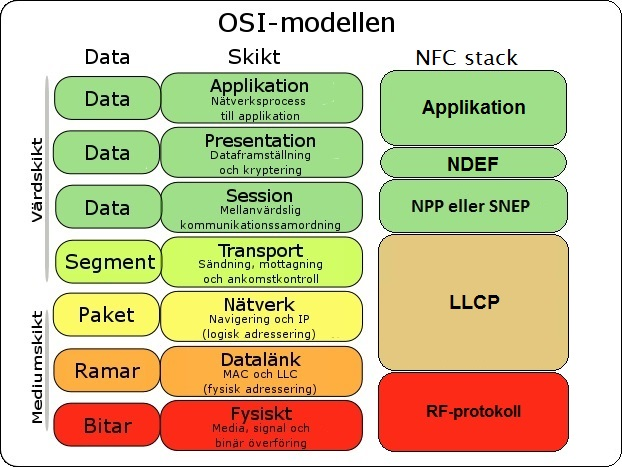
\includegraphics[scale=0.8]{NFC_stack.jpg}
\caption{NFC stack.}
\label{fig:NFC_stack}
\end{figure}

De översta fyra lagren implementeras i mjukvara vilka körs på mikrokontrollern då NFC-skölden endast har RF-protokollen implementerade. Då en mikrokontroller önskar nyttja RF(Radio Frequency)-protokollen behöver kommunikation ske mot NFC-skölden, denna funktionallitet åskådligörs via ett lager mellan LLCP och RF-protokoll och beskrivs också mellan dessa avsnitt.

\subsubsection{RF-protokoll-lagret}
De protokoll som specifierar den fysiska överföringen av NFC-meddelanden är implementerade i PN532 NFC/RFID Shield och behöver således inte utvecklas. Dock krävs styrning av de funktioner vilka RF-protokollen erbjuder, såsom att skicka eller att ta emot meddelanden. Detta sker genom kommunikation från mikrokontrollern till skölden och vilka kommandon som skickas beskrivs nedan.

\paragraph{Kontroll av RF-protokollens funktioner}
Skölden har en stor mängd kommandon som kan nyttjas och de som används av projektet beskrivs i avsnitt 3.3.2 (NFC för Arduino mha PN532 NFC/RFID Shield). Källkodsbiblioteket Embedded-PN532 implementerar de kommandon vilka ger den kontroll av skölden detta arbete söker, men de parametrarna vilka skickas med ett kommando har i viss grad modifierats. Detta gjordes i samband med att sessionslagret NPP byttes ut till förmån mot SNEP(se avsnitt 6.1.4).

De kommandon vilka anropas från att skölden startas upp till dess att data utbytes mot en aktiv NFC-enhet, beskrivs i tabell \ref{tab:PN532_kommandon}. Observera att kommandot SAMConfigure endast anropas vid uppstart av skölden och anropas inte igen såvida inte skölden startas om. Observera också att Kommando och Respons visas i hexadecimal teckenkodning.

%bild
%bildtext: Tabell XIV, omarbetat från applikation guide
\begin{figure}[H]
\centering
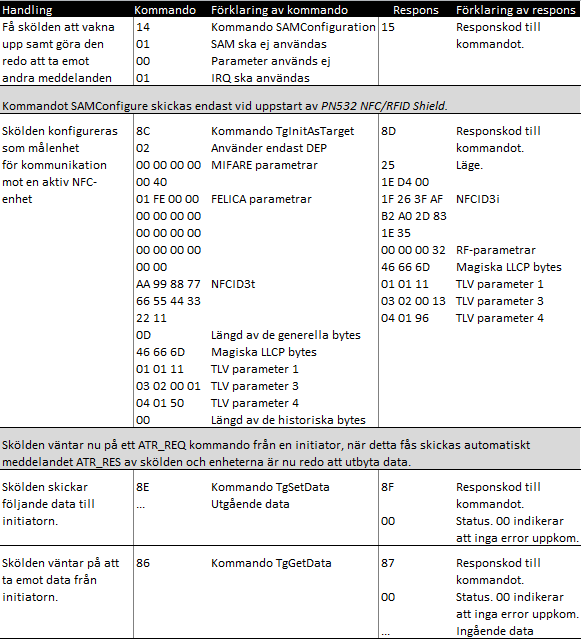
\includegraphics[scale=0.7]{PN532_kommandon.png}
\caption{Kommandon från skölden.}
\label{tab:PN532_kommandon}
\end{figure}

För att en ny uppkoppling ska ske mot en enhet måste kommandot TgInitAsTarget anropas och efter anropet väntar skölden på ett meddelande av typen ATR\_REQ från initiatorn. När ATR\_REQ inkommit returneras detta i svaret på TgInitAsTarget-kommandot, som det initiala meddelandet, och kan utläsas i tabell XIV efter de inledande bytsen 8D och 25.

\subsubsection{Kommunikation mellan Arduino och NFC-sköld}
Källkodsbilioteket Embedded-PN532 implementerar kommunikation mot skölden via SPI[källa], men valet att istället använda kommunikationstekniken I2C[källa] gjordes. Detts besut togs för att skölden i grundutförande använder I2C och för att I2C är enklare att förstå då den har en högre abstraktionsnivå än SPI. I2C använder buffrar till ut- och ingående meddelanden vilka manipuleras med hjälp av olika funktioner (metoder) och får på så sätt en högre abstraktionsnivå än SPI, som skickar och tar emot meddelanden direkt på kabeln en byte i taget. Nackdelen med att använda I2C är att buffrarna, vilka är fem till antalet, kan ta relativt stor del av det begränsade SDRAM- minnesutrymmet. För att kunna utbyta applikationsdata uppåt 200 bytes valdes en bufferstorlek på 256 bytes, vilket resulterar i en total SDRAM användning på 1280 bytes.

Följande stycke ska nog ligga i diskussion.
Att byta ut SPI mot I2C var relativt enkelt då det källkodsbibliotek som följde med PN532 NFC/RFID Shield fanns i två versioner, där den ena bygger på SPI och den andra bygger på I2C för kommunikation mot en Arduino. Dessvärre behövde I2Cs buffrar vara relativt stora, omkring 180 bytes styck, då skölden inte klarar att ta emot segmenterade meddelanden, men då Arduino Mega 2560 R3 har 8KB RAM-minne varvar 0.5KB består av mikrokontrollerns minneshanterare finns utrymme för att använda I2C.  

\subsubsection{LLCP-lagret}
Vid implementationen av LLCP-lagret används den officiella definitionen av protokollet som är utgivet av NFC-forum (källa). Android version 4.0 implementerar LLCP något annorlunda än Android version 2.3 vilket Embedded-PN532 är skrivet efter. Detta gjorde att befintlig kod för detta lagret behövde modifieras. Information direkt från Google kring hur protokollet är tolkat gick tyvärr inte att finna, men ett projekt hittades för kommunikation mot Android 4.0 genom att nyttja ett NFC-chip likt det som används i detta arbete(källa).  Det funna projektet var skrivet i programspråket Java och visar klart och tydligt hur LLCP ska användas för att skapa en länk mot en mobiltelefon med Android. Detta projekt används därför som en mall vid modifiering av LLCP-lagret i källkodsbibioteket Embedded-PN532. Bilden nedan visar hur server respektive klient nyttjar LLCP i (källa) projektet för att skapa samt stänga ned en länk då Android 4.0 används, och detta är också det förfarandet som Embedded-PN532 skrivs om till att utföra.

%bild: som visar hur server respektive klient nyttjar LLCP enligt java-man för att skapa samt stänga ned en länk. FINNS INTE ÄNNU!

\subsubsection{NPP- eller SNEP-lagret}
NPP är implementerat i Embedded-PN532 men då NPP är ett protokoll som nu har blivit utbytt, samt att det är relativt komplext och svårt att till fullo greppa, gjordes valet att byta ut detta till förmån för SNEP. Det nya protokollet SNEP är i förhållande till NPP är väldigt rättfram och enkelt att förstå. Detta val gjordes även då det i kommunikation mot Android fortfarande går det att använda NPP då Android-enheten faller tillbaka på det gamla protokollet om den känner av att det nya protokollet SNEP inte används. 

Eftersom data utbyts i båda riktningarna i kommunikationen har valet gjorts att ge låsenheten funktionalitet att agera både som klient och server, här betyder detta att låsenheten både kan skicka samt ta emot SNEP-förfrågningar. Den SNEP förfrågning vilket stöd har implementerats för är Put, vilken beskrivs i avsnitt 3.1.1.2 där också SNEP förklaras. 

Då låsenheten agerar som klient skickas en Put-förfrågan enligt figur KAKA där fältet Version har värdet 10 vilket anger att SNEP version 1,0 används. Vidare innehåller fältet Request värdet 02 vilket är den specifika koden som anger att detta är en Put-förfrågan och Length innehåller storleken av det NDEF-meddelande vilket huseras i fältet Information. Om överföringer lyckades kommer servern skicka svarsmeddelandet Success vilket indikerar att Put-förfrågan har genomförts, annars sänds ett SNEP-svar vilket fel som uppkom.
Figur KAKA. Figuren visar de värden vilka används i en Put-förfrågan. Delvis omarbetad från SNEP.

%bild
%bildtext: Figur KAKA. Figuren visar de värden vilka används i en Put-förfrågan. Delvis omarbetad från SNEP.

När låsenheten agerar som server väntar låsenheten på att ta emot en Put-förfrågan och då denna mottagits undersöks om förfrågans SNEP-version stödjs, vilken finns i fältet Version. Om versionen stödjs tas det mottagna NDEF-meddelandet om hand, vilket huseras i fältet Information, och svarsmeddelandet Success skickas till klienten. Om versionen inte stödjs eller något annat fel uppkommer avbryts kommunikationen och förloppet måste börja om.

\subsubsection{NDEF-lagret}
NDEF(NFC Data Exchange Format) är implementerat i Embedded-PN532 och biblioteket innehåller de funktioner som arbetet eftersöker, detta medför att NDEF-lagret inte har utvecklats vidare. 

Skriv om hur vi använder NDEF. Visa också med BILD

\subsubsection{Applikationen, den som snurrar i \texttt{loop()}}
Applikationen är utformad på sådant sätt att mikrokontrollern till en början 

skriv steg för steg vad som händer

\subsubsection{Fysisk implementering - är den aktuell?}
En prototyp där låsenheten fysiskt har implementeras i något form av lås bör färdigställas. Flertalet potentiella implementeringsmöjligheter finns bland annat genom att byta ut hela låshuset i en vanlig ytter- eller innerdörr,  använda en dörr med ett elektriskt lås och koppla in låsenheten mot denna eller att installera låsenheten i ett kassaskåp som har ett elektriskt lås. Om tid finnes för fysisk implementering ska den mest passande lösningen utredas. Om så behövs kommer låsenhetens formfaktor minskas för att möjliggöra lättare installation.

\subsection{Utveckling av mobilapplikationen}
Utvecklingen av applikationen för Android med stöd för NFC har bedrivits i iterativ form. En funktion har lagts till i taget för att sedan testas.
\begin{enumerate}
\item NFC-funktionaliteten. Som första steg utvecklades en applikation vars enda funktion var att skicka och ta emot information över NFC. Denna applikation utvecklades för att kommunisera med en annan app då mikrokontrollern i detta skede inte var redo för att kommunicera med en Android-telefon. För att implementera denna funktion använde vi Android Beam då det är den enda funktion moderna Android telefoner kan använda för att skicka och ta emot NFC-meddelanden.
\item NFC-funktionaliten utarbetades för att följa ovanstående kommunikationsprotokoll. Detta för att den skulle bli redo för mikrokontrollern när den var redo.
\item När kommunikationen var redo var mikrokontrollern långt ifrån klar att ta emot eller skicka meddelande. Därför gick utvecklingen vidare för att lägga till fler funktioner. Något sätt att kunna verifiera att rätt person hade tillgång till telefonen och därigenom dess nycklar behövde läggas till. Med anledning av detta implementereades PIN-kod med en bakomliggande timer för att få tillgång till applikationens alla funktioner.
\item När PIN-koden var på plats var applikationen redo för att okrypterat kunna låsa upp ett lås vars identifikationsnummer och upplåsningskommando behövde hårdkodas in i applikationen. Då detta är uppenbart är en lösning som inte går att skala upp utvecklades en bakomliggande databas med ansvar för att hålla reda nycklar och till vilket lås de hör till. Även om en lokal relationsdatabas användes då detta redan finns inbyggt stöd för i Android kan implementationen med stor sannolikhet göras effektivare med en så kallad Key-value-store. Databasen består av en tabell med låsets id som primär nyckel och upplåsningskommandot/nyckeln som andra kollumn.
\item Databasens funktioner integrerades i kommunikationsförloppet och en aktivitet med särskilt ansvar för att administrera databasen utvecklades. Aktiviteten kan lista paren, lägga till nya par och redigera gamla par.
\item När ovanstående steg var klart kunde man dela nycklar på ett begripligt sätt dock fanns ett behov av en automatisk funktion för delningen. Därför utvecklades en sådann automatisk funktion för delning mellan två mobilapplikationer. Delningen skedde genom att ett val av nyckel genomfördes för att sedan trycka på delning och hålla två telefoner mot varandra. NFC användes och en bekräftelse behövs för att den mottagande telefonen skall lägga till paret i dess databas.
\item Nästa steg var att få till en krypterad länk. Först implementerades kryptering i förloppet mellan två telefoner. Detta eftersom det är mycket lättare att använda de Java API som finns för kryptering än de som finns tillgängliga för en mikrokontroller som är skrivna i C.
\end{enumerate}

\subsection{Utveckling av en prototyp bestående av båda enhterna}
Skriv om hur vi fick ihop de båda till en produkt. Här är ju exempelvis kryptering väldigt relevant.

\section{Resultat}
Här bör vi beskriva resultaten och relatera dessa till kravspecifikationen
Detta kapitel ämnar beskriva resultaten av kandidatarbetet samt relatera dessa till den från början uppsatta kravspecifikationen. Såväl skallkrav som börkrav från kravspecifikationen behandlas.

\subsection{Produkten som helhet}
Projektet har resulterat i ett låssystem bestående av en mikrokontroller med NFC-kommunikation som exekverar mjukvara skriven i C++ och en Android-applikation skriven i Java. Enheterna kommunicerar via NFC. Android-applikationen kommunicerar genom Androids egna API för NFC-kommunikation, kallat Android Beam, och mikrokontrollern imiterar en Android-enhet med hjälp av en delvis egenutvecklad programvara. Kommunikationen sker i enligt det uppsatta kommunikationsprotkollet och kommunikationen är krypterad med RSA. Kommuniationsförloppet fungerar men är långsammare än det uppsatta kravet. Cirka 15 sekunder tar en lyckad upplåsning. 

\subsection{Mobilapplikationen}
Arbetet med Android-applikationen har resultaterat i en användbar men funktionsrik applikation. Applikationen uppfyller alla de skallkrav samt majoriteten av de börkrav som togs fram innan utvecklandet utav applikationen. De börkrav som inte uppfylls är att alla versioner av Android inte stödjs samt att applikationen inte har någon möjlighet att konfigurera låsmodulen. Sammanfattningsvis följer en lista av de krav applikationen klarar och inte klarar. Listan följs av en mer ingående beskrivning av applikationen.
\begin{itemize}
\item Applikationen följer Jacob Nielsen’s heuristik
\item Applikationen är noga testad och har inga kända buggar.
\item Applikationen fungerar inte på alla NFC-telefoner. Detta eftersom från och med Android 4.0 ändrades kommunikationen radikalt. Därför stödjs bara 4.0 eller senare.
\item Nycklar kan delas med andra applikationer över NFC.
\item Applikationen kräver personverifiering med hjälp av PIN-kod.
\item Applikationen har ingen möjlighet att konfigurera om låsenheten.
\end{itemize}

Mobilapplikationen bör vara lättförståelig och mycket enkel att hantera då det är användandet av en vanlig metallnyckel som ska konkurreras med. Vidare bör inga kända buggar finnas samt att nycklar bör kunna delas med andra mobiltelefoner som har mobilapplikationen installerad. Mobilapplikatonen bör även tillhandhålla någon form av personverifiering, t.ex. PIN-kod.

Applikationen består av ca 2000 rader Java-kod och till det ca 500 rader xml-definerade gränssnitt. 
kort överblick, består av 2000 rader Java-kod.

\subparagraph{Övergripande design}
Applikationen är skapad för att så enkelt som möjligt tillhandahålla de funktioner användaren behöver. Med en enkel design uppstår inga onödiga svårigheter och med återkommande typsnitt, färger och platformskonventioner uppstår en trygghet i designen. De aktiviteter som har menyer visas som actionbars för att öka synligheten, annars visas de endast då menyknappen trycks ner.

%bilder
%bildtext: Figur 1 till 6.

Figurerarna 1 till 6 ovan visar i tur och ordning aktiviterna Login, Main, Success, Settings, Password och Keys.
Följande stycken ämnar beskriva dem och dess funktion.

\subparagraph{Login}
Login är den första aktiviteten som en användare av Android-applikationen möts av. Den huvudsakliga funktionen av denna aktivitet är att förhindra att applikationen kan användas av oönskade användare. Den fungerar som en port till övriga applikationen genom att implementera ett system för personverifiering med hjälp av PIN-kod. Ges inte rätt PIN-kod går inte övriga delar av applikationen att nå. När korrekt PIN-kod har angivits startas en timer. Timern loggar ut användaren igen efter en bestämd tid. 

\subparagraph{Main}
När användaren angett PIN-kod möts han av nästa aktivitet, Main. Main är aktiviten hela applikationen bygger runt. Den är ansvarig för kommunikationen och att automatiskt skicka rätt NDEF-meddelande utgående från det senaste mottagna meddelandet. Detta sker helt enligt ovanstående kommunikationsprotokoll. Användaren informeras om förloppet med hjälp av en textvy, lokaliserad nedtill. När kommunikationen har nått sitt mål, en upplåst dörr, eller om detta inte skulle ske skickas användaren vidare till Success-aktiviten alternativt Denied-aktiviteten. Är det inkommande meddelandet däremot delning av en nyckel kommer det upp en bekräftelseruta där en bekräftelse från användaren krävs innan nyckeln läggs till i databasen.

Om användaren har behov av av att ändra inställningar för applikationen trycker denne på Settings-knappen lokaliserad längst ned på skärmen för att komma till Settings-aktiviteten.

\subparagraph{Success och Denied}
Success-aktiviteten har till uppgift att visa för användaren att upplåsningen lyckades. Vid ett anrop visas aktiviteten bara en kortare stund för att sedan avslutas och applikationen går tillbaka till Main-aktiviten. Förutom Success finns det även en liknande aktivitet kallad Denied. Den har till uppgift att visa vad som gick snett om något går snett vid låsförfarandet. För övrigt fungerar den på samma sätt som Success.

\subparagraph{Settings}
Settings-aktivteten nås via knappen längst ner i Main. Aktiviten har till uppgift att rada de inställningar som finns att göra. Prototypen innehåller endast två sådanna men aktivten är förberedd för fler. Trycker användaren på knapparna kommer denne vidare till aktiviterna Password respektive Keys.

\subparagraph{Password}
Denna aktivitet har den enkla uppgiften att ändra PIN-kod. För att kunna ändra PIN-kod krävs att den gamla anges korrekt.

\subparagraph{Keys}
Sist men inte minst finns aktiviten Keys. Huvuduppgiften för denna aktivitet, som är applikationens nästa största, är att ansvara för hanteringen av nyckelpar. Bakom aktiviten ligger en lokal relationsdatabas av SQLite-typ som är ansvarig för att lagra nyckelparen. De databasfunktioner aktiviten ger ett ovanliggande skal till är att lista alla par, redigera ett par, ta bort ett, lägga till nya, söka och att dela med andra smarta telefoner med applikationen installerad.

Längst upp på skärmen återrfinns en bläddringsbar vy med alternativknappar. Vyn listar de nyckelpar som finns i databasen och det går att välja en i taget. När en knapp är vald går det att använda knapparna för att ta bort nyckelparet från databasen eller för att dela den genom knappen nedtill. Delningsfunktionen skickar användaren vidare till en annan skärm. Förs telefonen då mot en annan smarttelefon är det möjligt att dela paret genom att röra skärmen. Nedtill finns också knappar för att skapa nya nyckelpar och för att söka bland befintliga. Popup-fönster dyker upp för dessa uppgifter.

\subsection{Låsenheten}
Den slutliga låsenheten kan kommunicera mot mobiltelefoner med Android 4.0 eller senare. De mobiltelefoner vilka låsenheten har kommunicerat mot är HTC One X, Samsung galaxy S3 och LG optimus L5. Vidare stödjer låsenheten säker kommunikation via krykrypteringsalgoritmen RSA med 512-bitar stora nycklar. Skölden, PN532 NFC/RFID Shield, har kompletterats med en mindre diod-krets vilken indikerar om låset låstes upp eller ej.

Mikrokontrollern stödjer den funktionallitet vilken krävs för att hantera kommunikation med skölden. En minimalistisk implementaion, dvs de kommandon som utgör kärnan vid aktiv kommunikation, används. Kommunikation mellan mikrokontroller och sköld utförs med I2C som kommunikationsprotokoll.

Låsenheten  erbjuder ett adekvat stöd för aktiv NFC-kommunikation. Den tillhandahållna NFC-stacken består av 
minimalistiska implementationer av NDEF, SNEP och LLCP. De avkall vilka har gjorts har resulterat i begränsningar på mängden data vilket kan skickas mellan NFC-enheterna. Gränsen på data från applikations-lager ligger på 250-bytes per sändning. När diverse headers plockas bort resulterar detta i en datamängd på ….. för ren applikationsdata. Vid sändning kan en datamängd på 163 bytes skickas vilket ger 139 bytes för ren appliationsdata.  LTO har satts till 800ms vilket är tillräckligt även för de långsammare Android telefonerna.

Låsenheten stödjer dekryptering av 512-bitars RSA. Detta är det delmoment i mikrokontrollerns arbetsbörda som tar absolut längst tid. Dekrypteringen tar 3.2 sekunder av den totala körningstiden som beräknats till ca 15 sekunder på Arduino Mega 2560. 

I befintlig implementation är upplåsningsnyckel hårdkodad och inte konfigurearbar. För att konfigurera krävs att drivrutiner modifieras, kompileras och laddas upp på mikrokontrollern. 

För att sänka energiförbrukningen försätts låsenheten i ett strömsparläge då dess tjänster inte behövs. Mikrokontrollern väcks av en signal som skölden skickar när den detekterar ett NFC fält. Om även mikrokontrollern tillåts vara aktiv hela tiden fås en nominell strömförbrukning på ….. . Med strömsparfunktioner landar den på …...

Mikrokontrollerns drivrutiner omfattas av 2500 rader C++ kod. Kompilerat och uppladdat på Arduinon tar detta 28880 bytes av de totalt 256kbytes som finns tillgängliga. Runtime kontroller av användandet av SDRAM har uppgått till maximalt 4209 bytes av 8kbytes.  

\section{Diskussion}

\subsection{Produkten}

\subsection{Arduino}

\subsection{Mobilapplikationen}

\section{Slutsats}

\section*{Referenser}

\section*{Bilagor}

\end{document}
